\documentclass[compress,trans,9pt]{beamer}
% \documentclass[9pt]{beamer}
%\documentclass[compress,9pt,usenames,dvipsnames]{beamer}
% \usepackage[utf8]{inputenc}
% \includeonlyframes{current}
\setbeamercovered{dynamic}
\usepackage{etex}
\usepackage{graphicx,url,psfrag}
\usepackage{tikz}
\usetikzlibrary{
  decorations.pathreplacing,
  calc,
  decorations.fractals,
  through,
  shapes,
  patterns,
  arrows.meta,
  decorations.pathreplacing,
  arrows,
  shapes,
  mindmap
}
\usepackage[center]{subfigure}
\usepackage{enumerate}
\usepackage[makeroom]{cancel}
\usepackage{mathtools}
\usepackage{graphbox}
\usepackage{amssymb}
% \usepackage[showframe]{geometry}
% \usepackage{enumitem}

%
% for warning sign
%
\usepackage{stackengine}
\usepackage{scalerel}
\usepackage{xcolor}
\newcommand\dangersign[1][2ex]{%
  \renewcommand\stacktype{L}%
  \scaleto{\stackon[1.3pt]{\color{red}$\triangle$}{\tiny !}}{#1}%
}
% %  The following is to show codes:
\usepackage{listings}
% \usepackage{color}
\usepackage{colortbl}
\usepackage{dbt}

\definecolor{dkgreen}{rgb}{0,0.6,0}
\definecolor{gray}{rgb}{0.5,0.5,0.5}
\definecolor{mauve}{rgb}{0.58,0,0.82}

% \definecolor{deepblue}{rgb}{0,0,0.5}
% \definecolor{deepred}{rgb}{0.6,0,0}
% \definecolor{deepgreen}{rgb}{0,0.5,0}
% \lstset{
%   language=Python,
%   backgroundcolor=\color{red},  % choose the background color. You must add \usepackage{color}
%   % backgroundcolor=\color{background},  % choose the background color. You must add \usepackage{color}
%   basicstyle=\footnotesize,
%   otherkeywords={self},
%   keywordstyle=\ttb\color{deepblue},
%   emph={MyClass,__init__},
%   emphstyle=\ttb\color{deepred},
%   stringstyle=\color{deepgreen},
%   commentstyle=\color{red},  %%%%%%%%
%   frame=tb,
%   showstringspaces=false
% }
%
% \lstdefinestyle{Python}{
%     language        = Python,
%     basicstyle      = \footnotesize,
%     keywordstyle    = \color{blue},
%     keywordstyle    = [2] \color{red}, % just to check that it works
%     stringstyle     = \color{green},
%     commentstyle    = \color{red}\ttfamily
% }

\lstset{frame=tb,
  language=Java,
  aboveskip=3mm,
  belowskip=3mm,
  showstringspaces=false,
  columns=flexible,
  basicstyle={\small\ttfamily},
  numbers=none,
  numberstyle=\tiny\color{gray},
  keywordstyle=\color{blue},
  commentstyle=\color{dkgreen},
  stringstyle=\color{mauve},
  breaklines=true,
  breakatwhitespace=true,
  tabsize=3
}
\lstset{language=Java}

\lstset{ %
  language=R,                     % the language of the code
  basicstyle=\footnotesize,       % the size of the fonts that are used for the code
  numbers=left,                   % where to put the line-numbers
  numberstyle=\tiny\color{gray},  % the style that is used for the line-numbers
  stepnumber=1,                   % the step between two line-numbers. If it's 1, each line
                                  % will be numbered
  numbersep=5pt,                  % how far the line-numbers are from the code
  backgroundcolor=\color{background},  % choose the background color. You must add \usepackage{color}
  showspaces=false,               % show spaces adding particular underscores
  showstringspaces=false,         % underline spaces within strings
  showtabs=false,                 % show tabs within strings adding particular underscores
  frame=single,                   % adds a frame around the code
  rulecolor=\color{black},        % if not set, the frame-color may be changed on line-breaks within not-black text (e.g. commens (green here))
  tabsize=2,                      % sets default tabsize to 2 spaces
  captionpos=b,                   % sets the caption-position to bottom
  breaklines=true,                % sets automatic line breaking
  breakatwhitespace=false,        % sets if automatic breaks should only happen at whitespace
  title=\lstname,                 % show the filename of files included with \lstinputlisting;
                                  % also try caption instead of title
  keywordstyle=\color{blue},      % keyword style
  commentstyle=\color{dkgreen},   % comment style
  stringstyle=\color{mauve},      % string literal style
  escapeinside={\%*}{*)},         % if you want to add a comment within your code
  morekeywords={*,...}            % if you want to add more keywords to the set
}
% \usepackage[usenames,dvipsnames]{color}
% \lstset{
%   language=Python,                     % the language of the code
%   basicstyle=\footnotesize,       % the size of the fonts that are used for the code
%   numbers=left,                   % where to put the line-numbers
%   numberstyle=\tiny\color{gray},  % the style that is used for the line-numbers
%   stepnumber=1,                   % the step between two line-numbers. If it's 1, each line
%                                   % will be numbered
%   numbersep=5pt,                  % how far the line-numbers are from the code
%   backgroundcolor=\color{background},  % choose the background color. You must add \usepackage{color}
%   showspaces=false,               % show spaces adding particular underscores
%   showstringspaces=false,         % underline spaces within strings
%   showtabs=false,                 % show tabs within strings adding particular underscores
%   frame=single,                   % adds a frame around the code
%   rulecolor=\color{black},        % if not set, the frame-color may be changed on line-breaks within not-black text (e.g. commens (green here))
%   tabsize=2,                      % sets default tabsize to 2 spaces
%   captionpos=b,                   % sets the caption-position to bottom
%   breaklines=true,                % sets automatic line breaking
%   breakatwhitespace=false,        % sets if automatic breaks should only happen at whitespace
%   title=\lstname,                 % show the filename of files included with \lstinputlisting;
%                                   % also try caption instead of title
%   keywordstyle=\ttb\color{blue},      % keyword style
%   commentstyle=\color{dkgreen},   % comment style
%   stringstyle=\color{mauve},      % string literal style
%   escapeinside={\%*}{*)},         % if you want to add a comment within your code
%   morekeywords={*,...}            % if you want to add more keywords to the set
% }

% \usepackage[dvipsnames]{xcolor}
% \newcommand{\Cross}{\mathbin{\tikz [x=1.4ex,y=1.4ex,line width=.2ex] \draw (0,0) -- (1,1) (0,1) -- (1,0);}}%
\newcommand{\Crossme}[1]{\!\!
\tikz [black,x=1.1em,y=1.1em,line width=.4ex]
\draw (-0.5,-0.5) -- (0,0) node {\footnotesize #1} -- (0.5,0.5) (0.5,-0.5) -- (-0.5,0.5);}%
\newcommand{\Checkme}[1]{\!\!
\tikz [x=1.1em,y=1.1em,line width=.4ex]
\draw [black] (0,0.7) -- (0.3,0) --(0.9,1.0) (0.5,0.5) node {\footnotesize #1};}
% \beamerdefaultoverlayspecification{<+-| alert@+>} %(this will show line by line)
\beamerdefaultoverlayspecification{<+->} %(this will show line by

% \usepackage{natbib}
% \input{../myMathSymbols.tex}
% \newcommand{\tlMr}[4]{\:{}^{\hspace{0.2em}#1}_{#2} \hspace{-0.1em}#3_{#4}}

% Smiley face\Smiley{} \Frowny{}
\usepackage{marvosym}
% -------------------------------------------------
%  Set directory for figs
% -------------------------------------------------
\usepackage{grffile}
\graphicspath{{Codes/}}
% -------------------------------------------------
%  Define colors
% -------------------------------------------------
\def\refcolor{cyan}
\newcommand{\myref}[1]{\small {\em #1}}
\def\excolor{brown}
% \usepackage{color}
% \usepackage[dvipsnames]{xcolor}


% % % Define danger sign
\newcommand*{\TakeFourierOrnament}[1]{{%
\fontencoding{U}\fontfamily{futs}\selectfont\char#1}}
\newcommand*{\danger}{\TakeFourierOrnament{66}}


% -------------------------------------------------
%  Define short-hand symbols.
% -------------------------------------------------
\newcommand{\B}{\textbf{B}}
\newcommand{\PP}{\mathbb{P}}
\newcommand{\E}{\mathbb{E}}
\newcommand{\D}{\mathbb{D}}
\newcommand{\W}{\dot{W}}
\newcommand{\ud}{\ensuremath{\mathrm{d}}}
\newcommand{\Ceil}[1]{\left\lceil #1 \right\rceil}
\newcommand{\Floor}[1]{\left\lfloor #1 \right\rfloor}
\newcommand{\sgn}{\text{sgn}}
\newcommand{\Lad}{\text{L}_{\text{ad}}^2}
\newcommand{\SI}[1]{\mathcal{I}\left[#1 \right]}
\newcommand{\SIB}[2]{\mathcal{I}_{#2}\left[#1 \right]}
\newcommand{\Indt}[1]{1_{\left\{#1 \right\}}}
\newcommand{\LadInPrd}[1]{\left\langle #1 \right\rangle_{\text{L}_\text{ad}^2}}
\newcommand{\LadNorm}[1]{\left|\left|  #1 \right|\right|_{\text{L}_\text{ad}^2}}
\newcommand{\Norm}[1]{\left|\left|  #1   \right|\right|}
\newcommand{\Ito}{It\^{o} }
\newcommand{\Itos}{It\^{o}'s }
\newcommand{\spt}[1]{\text{supp}\left(#1\right)}
\newcommand{\InPrd}[1]{\left\langle #1 \right\rangle}
\newcommand{\mr}{\textbf{r}}
\newcommand{\Ei}{\text{Ei}}
\newcommand{\arctanh}{\operatorname{arctanh}}
\newcommand{\ind}[1]{\mathbb{I}_{\left\{ {#1} \right\} }}
\newcommand{\Var}{\text{Var}}
\newcommand{\Cov}{\text{Cov}}
\newcommand{\Corr}{\text{Corr}}

\newcommand{\baseurl}[1]{\footnotesize\url{http://math.emory.edu/~lchen41/teaching/2020_Spring/#1}}


\newcommand*\mystrut[1]{\vrule width0pt height0pt depth#1\relax} % adding vertical space

\DeclareMathOperator{\esssup}{\ensuremath{ess\,sup}}

\newcommand{\steps}[1]{\vskip 0.3cm \textbf{#1}}
\newcommand{\calB}{\mathcal{B}}
\newcommand{\calC}{\mathcal{C}}
\newcommand{\calD}{\mathcal{D}}
\newcommand{\calE}{\mathcal{E}}
\newcommand{\calF}{\mathcal{F}}
\newcommand{\calG}{\mathcal{G}}
\newcommand{\calK}{\mathcal{K}}
\newcommand{\calH}{\mathcal{H}}
\newcommand{\calI}{\mathcal{I}}
\newcommand{\calL}{\mathcal{L}}
\newcommand{\calM}{\mathcal{M}}
\newcommand{\calN}{\mathcal{N}}
\newcommand{\calO}{\mathcal{O}}
\newcommand{\calT}{\mathcal{T}}
\newcommand{\calP}{\mathcal{P}}
\newcommand{\calR}{\mathcal{R}}
\newcommand{\calS}{\mathcal{S}}
\newcommand{\calV}{\mathcal{V}}
\newcommand{\bbC}{\mathbb{C}}
\newcommand{\bbN}{\mathbb{N}}
\newcommand{\bbP}{\mathbb{P}}
\newcommand{\bbZ}{\mathbb{Z}}
\newcommand{\myVec}[1]{\overrightarrow{#1}}
\newcommand{\sincos}{\begin{array}{c} \cos \\ \sin \end{array}\!\!}
\newcommand{\CvBc}[1]{\left\{\:#1\:\right\}}
\newcommand*{\one}{{{\rm 1\mkern-1.5mu}\!{\rm I}}}

\newcommand{\OneFrame}[1]{
\begin{enumerate}\item[#1] \phantom{av} \\[20em]\vfill\phantom{av}\myEnd\end{enumerate}}

\newcommand{\bH}{\ensuremath{\mathrm{H}}}
\newcommand{\Ai}{\ensuremath{\mathrm{Ai}}}

\newcommand{\R}{\mathbb{R}}
\newcommand{\myEnd}{\hfill$\square$}
\newcommand{\myQED}{\hfill\textcolor{lgtblue}{$\blacksquare$}}
\newcommand{\ds}{\displaystyle}
\newcommand{\Shi}{\text{Shi}}
\newcommand{\Chi}{\text{Chi}}
\newcommand{\Erf}{\ensuremath{\mathrm{erf}}}
\newcommand{\Erfc}{\ensuremath{\mathrm{erfc}}}
\newcommand{\He}{\ensuremath{\mathrm{He}}}
\newcommand{\Res}{\ensuremath{\mathrm{Res}}}

\newcommand{\mySeparateLine}{\begin{center}
 \makebox[\linewidth]{\rule{0.6\paperwidth}{0.4pt}}
\end{center}}

\theoremstyle{definition}
% \newtheorem{definition}[theorem]{Definition}
% \newtheorem{hypothesis}[theorem]{Hypothesis}
\newtheorem{assumption}[theorem]{Assumption}

\theoremstyle{plain}
% \newtheorem{theorem}{Theorem}
% \newtheorem{corollary}[theorem]{Corollary}
% \newtheorem{lemma}[theorem]{Lemma}
\newtheorem{proposition}[theorem]{Proposition}

\mode<presentation>
{
%      \usetheme{Warsaw}
%     \usetheme{JuanLesPins}
%  \usetheme{Hannover}
%  \usetheme{Montpellier}
   \useoutertheme{default}
  % or ...

  \setbeamercovered{transparent}
  % or whatever (possibly just delete it)
 \setbeamertemplate{frametitle}{
  \begin{centering}
    \color{blue}
    {\insertframetitle}
    \par
  \end{centering}
  }
}
\usefoottemplate{\hfill \insertframenumber{}}
% \inserttotalframenumber

\usepackage[english]{babel}
% or whatever

% \usepackage[latin1]{inputenc}
% or whatever

\usepackage{times}
\usepackage[T1]{fontenc}
% Or whatever. Note that the encoding and the font should match. If T1
% does not look nice, try deleting the line with the fontenc.

% \DeclareMathOperator{\Lip}{Lip}
\DeclareMathOperator{\lip}{l}
% \DeclareMathOperator{\Vip}{\overline{v}}
% \DeclareMathOperator{\vip}{\underline{v}}
% \DeclareMathOperator{\vv}{v}
% \DeclareMathOperator{\BC}{BC}
% \DeclareMathOperator{\CH}{CD}

\usepackage{pgfpages}
% \setbeameroption{show notes}
% \setbeamertemplate{note page}[plain]
% \setbeameroption{second mode text on second screen=right}
% \setbeameroption{show notes on second screen=right}
%
\title % (optional, use only with long paper titles)
{
Math 362: Mathematical Statistics II
}

% \subtitle
% {Research Plan} % (optional)

\author{Le Chen\\
\url{le.chen@emory.edu}\\
\url{chenle02@gmail.com}\\[2em]
Emory University\\
Atlanta, GA\\[2em]
\textcolor{gray}{\small Last updated on Spring 2021}\\
\textcolor{gray}{\small Last compiled on \today}
}
\institute[Emory University]
{%
\vspace{3em}
% \pgfuseimage{UNLV}
 }
 \vfill
% - Use the \inst command only if there are several affiliations.
% - Keep it simple, no one is interested in your street address.

% \date[Talk at Karlsruhe] % (optional)
% {\today }
 \date[Columbus]{
   2021 Spring\\[1em]
   Creative Commons License\\
   (CC By-NC-SA)
 }

\subject{}
% This is only inserted into the PDF information catalog. Can be left
% out.

% If you have a file called "university-logo-filename.xxx", where xxx
% is a graphic format that can be processed by latex or pdflatex,
% resp., then you can add a logo as follows:

% \pgfdeclareimage[height=0.8cm]{UNLV}{figs/UNLV-186.png}

% Delete this, if you do not want the table of contents to pop up at
% the beginning of each subsection:
% \AtBeginSubsection[]
% {
%   \begin{frame}<beamer>{Outline}
%     \tableofcontents[currentsection,currentsubsection]
%   \end{frame}
% }


% If you wish to uncover everything in a step-wise fashion, uncomment
% the following command:

% \beamerdefaultoverlayspecification{<+->}
% % % % % % % % % % % % % % % % % % %
%  Define a block
% % % % % % % % % % % % % % % % % % %
\newenvironment<>{problock}[1]{%
  \begin{actionenv}#2%
      \def\insertblocktitle{#1}%
      \par%
      \mode<presentation>{%
        \setbeamercolor{block title}{fg=white,bg=olive!95!black}
       \setbeamercolor{block body}{fg=black,bg=olive!25!white}
       \setbeamercolor{itemize item}{fg=white!20!white}
       \setbeamertemplate{itemize item}[triangle]
     }%
      \usebeamertemplate{block begin}}
    {\par\usebeamertemplate{block end}\end{actionenv}}

\newenvironment<>{assblock}[1]{%
  \begin{actionenv}#2%
      \def\insertblocktitle{#1}%
      \par%
      \mode<presentation>{%
        \setbeamercolor{block title}{fg=white,bg=green!50!black}
       \setbeamercolor{block body}{fg=black,bg=green!10}
       \setbeamercolor{itemize item}{fg=green!80!black}
       \setbeamertemplate{itemize item}[triangle]
     }%
      \usebeamertemplate{block begin}}
    {\par\usebeamertemplate{block end}\end{actionenv}}


\newcommand{\mySection}[1]{\section{\S\: #1}\begin{frame}{\myChapter}\tableofcontents[currentsection]\end{frame}}

\AtBeginSection[]
  {
     \begin{frame}<beamer>
     \frametitle{Plan}
     \tableofcontents[currentsection]
     \end{frame}
  }


\begin{document}

\AtBeginSection[]
  {
     \begin{frame}<beamer>
     \frametitle{Plan}
     \tableofcontents[currentsection]
     \end{frame}
  }


%-------------- start slide -------------------------------%{{{
\begin{frame}[noframenumbering]
  \titlepage
\end{frame}
%-------------- end slide -------------------------------%}}}


% \begin{frame}{Outline}
%   \tableofcontents
%   % You might wish to add the option [pausesections]
% \end{frame}



\newcommand{\myChapter}{Chapter 11. Regression}

%-------------- start slide -------------------------------%{{{
\begin{frame}
\begin{center}
\huge
\myChapter
\end{center}
\end{frame}
%-------------- end slide -------------------------------%}}}
\mySection{11.1 Introduction}
%-------------- start slide -------------------------------%{{{ 11.4
\begin{frame}
	% {\S\: 11.1 Introduction}
	\begin{center}
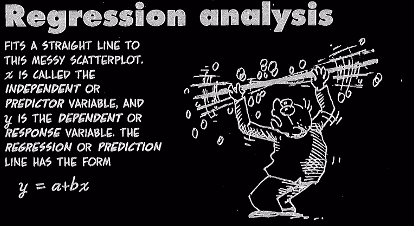
\includegraphics[scale=2]{cartoon_guide_regression-neg.png}
\vspace{2em}
\footnotesize
\url{https://madhureshkumar.wordpress.com/}
% 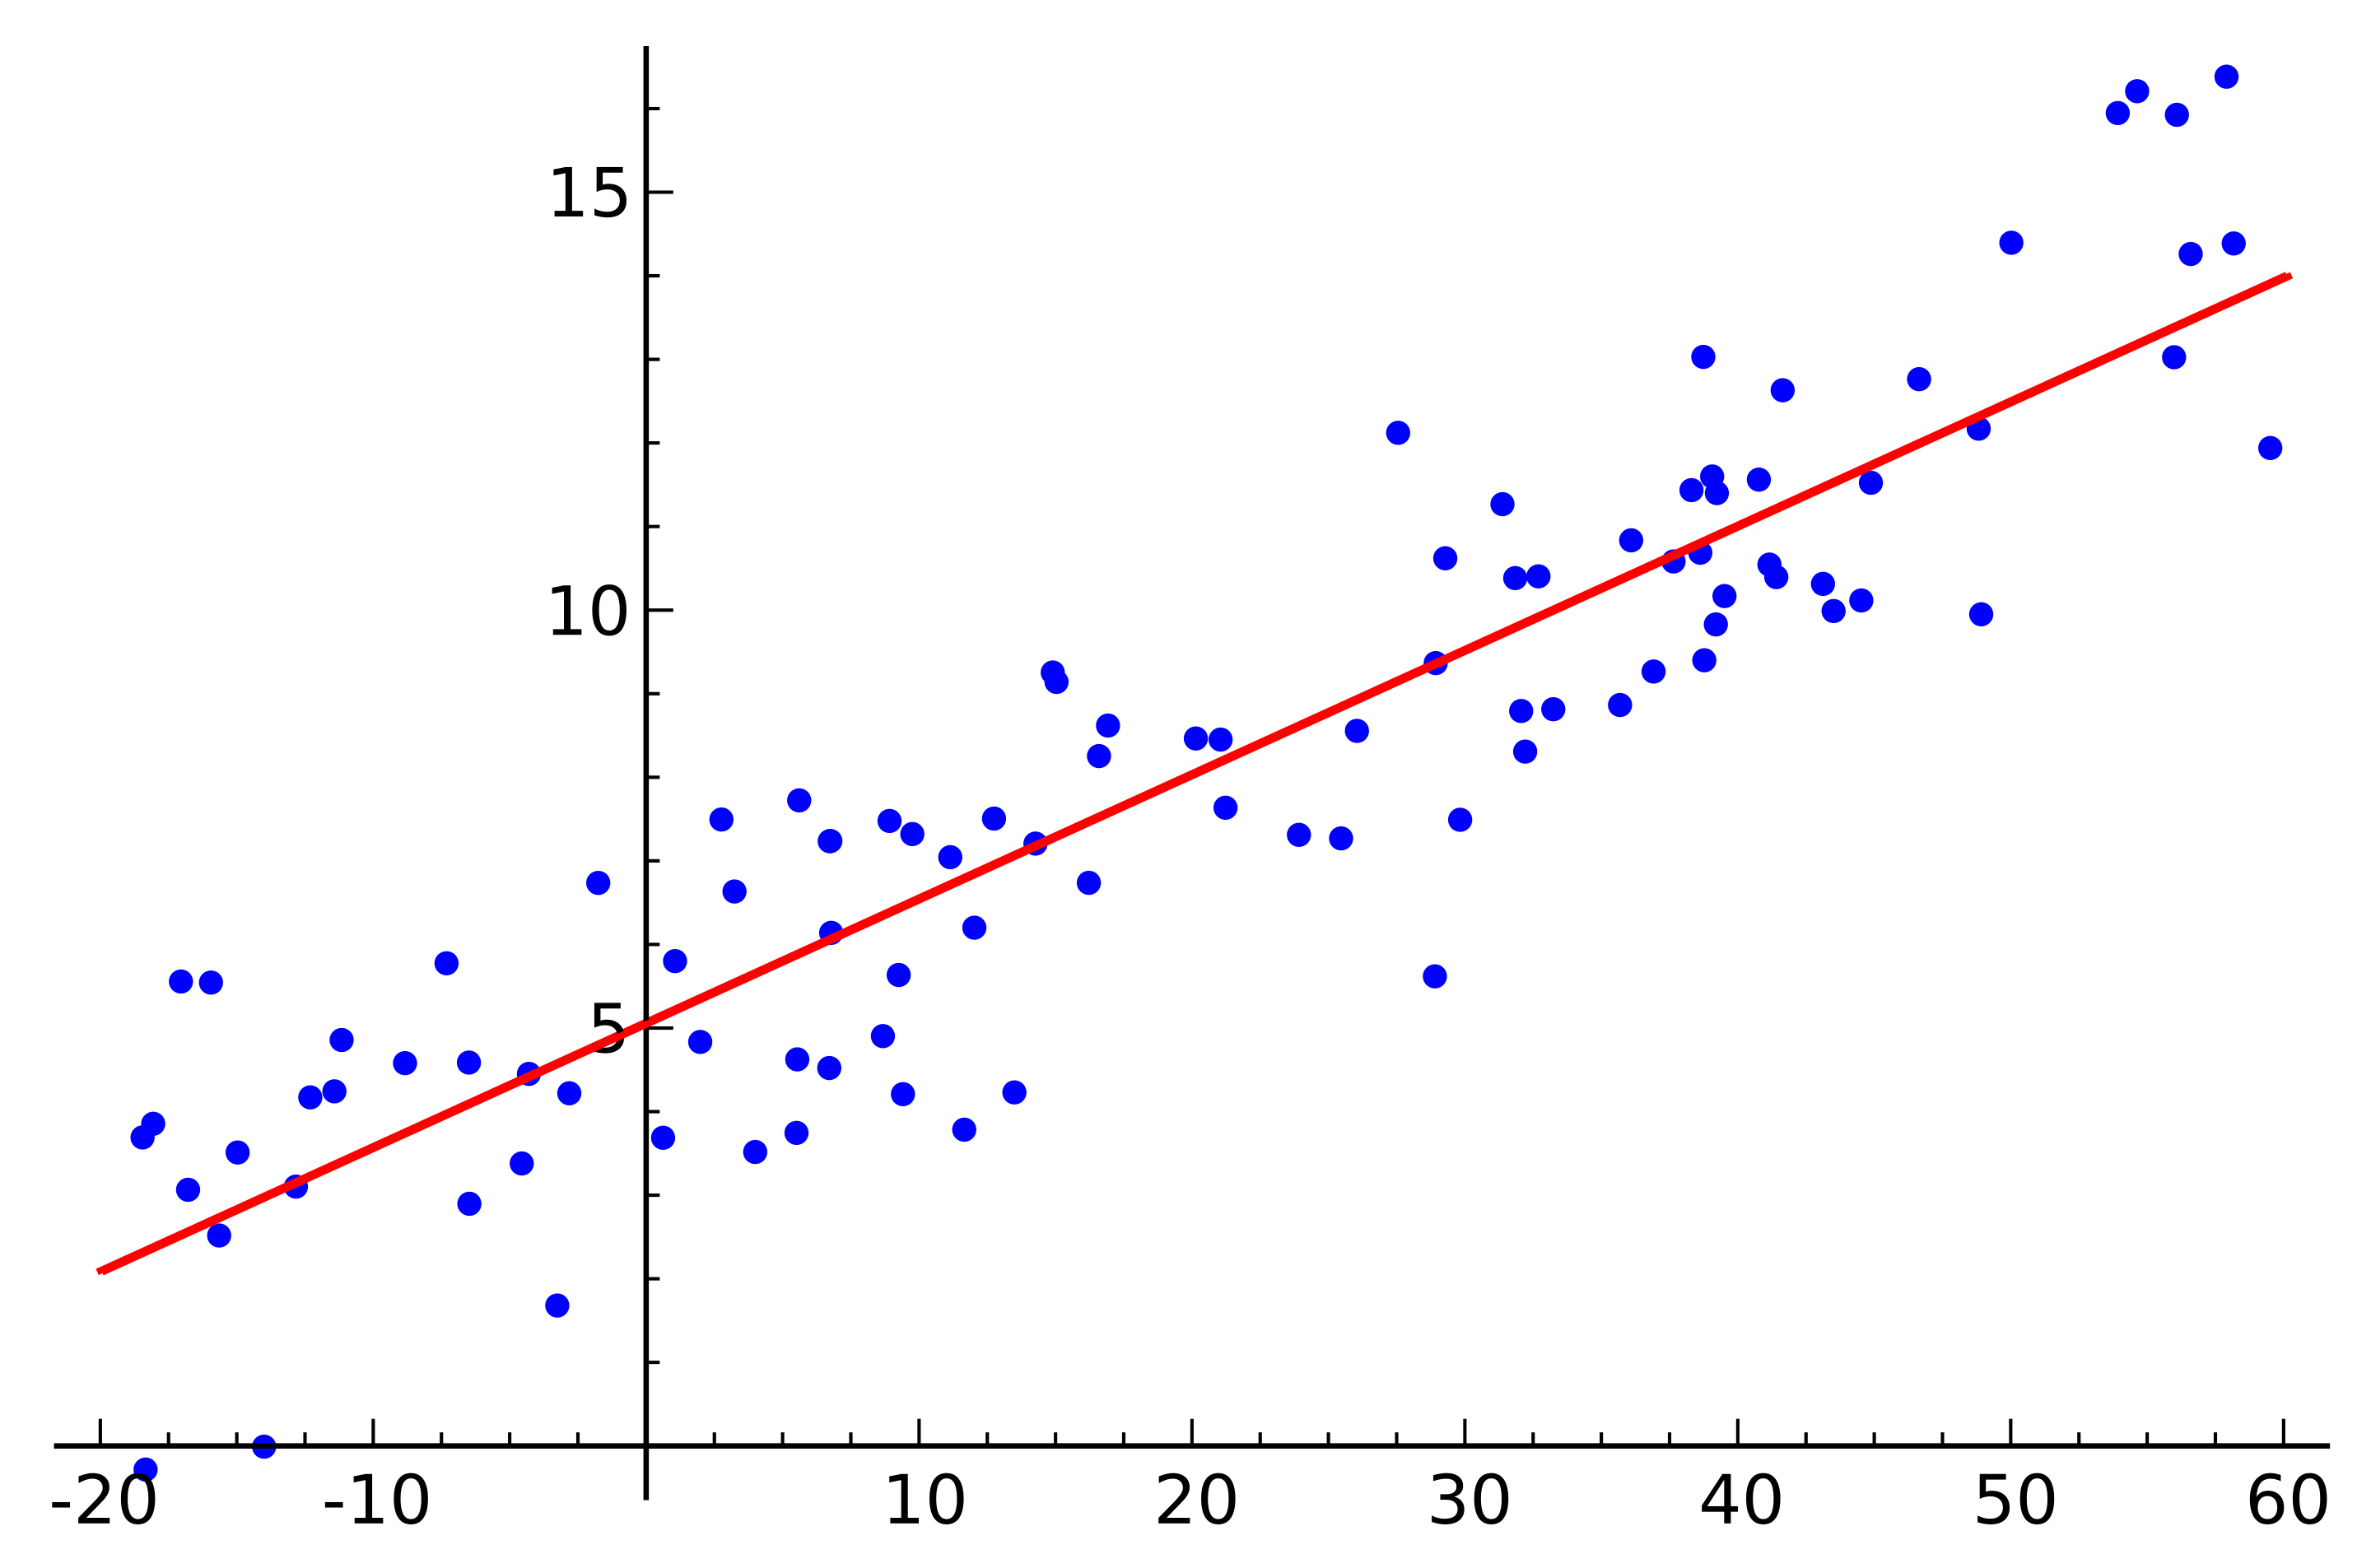
\includegraphics[scale=0.07]{2880px-Linear_regression.svg.png}
	\end{center}
\end{frame}
%-------------- end slide -------------------------------%}}}
%-------------- start slide -------------------------------%{{{ 11.5
\begin{frame}
	\centering
	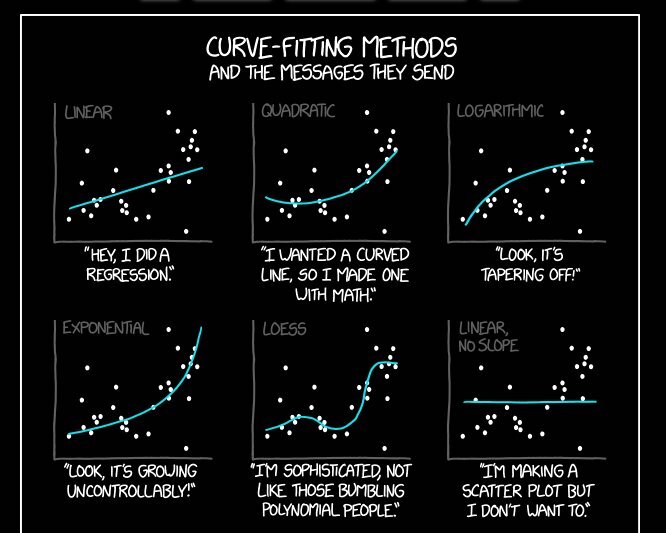
\includegraphics[scale=0.34]{xkcd_Curve_fitting2-neg.jpg}
	\\
	\footnotesize \url{https://xkcd.com/}
	% 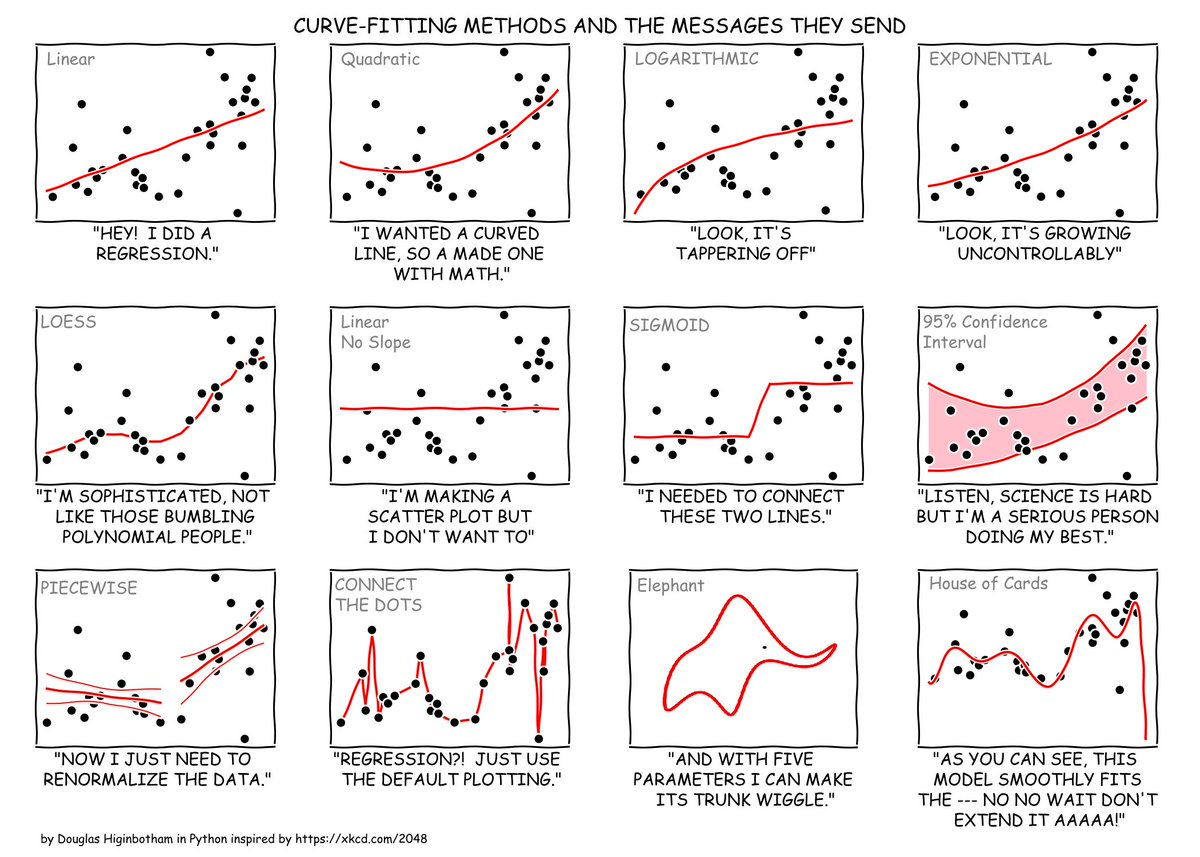
\includegraphics[scale=0.25]{xkcd_Curve_fitting.jpg}
\end{frame}
%-------------- end slide -------------------------------%}}}
%-------------- start slide -------------------------------%{{{ 11.6
\begin{frame}[fragile]{Three ways to view the same thing}

	\begin{enumerate}
		\item[]
			\[(x_1,y_1),\cdots, (x_n,y_n)\]
		\item Purely data, no probability structure assumed.
			\vfill
		\item[]
			\[(x_1,Y_1),\cdots,(x_n,Y_n)\]
		\item A random sample of size $n$, where $Y_i$ follows a distribution depending on $x_i$ which is 
			deterministic.
			\vfill
		\item[]
			\[
			(X_1,Y_1),\cdots,(X_n,Y_n)
			\]
		\item A random sample of size $n$, where $(X_i,Y_i)$ follow some joint distribution.
	\end{enumerate}
\end{frame}
%-------------- end slide -------------------------------%}}}

\mySection{11.2 The Method of Least Squares}
%-------------- start slide -------------------------------%{{{ 11.18
\begin{frame}
	% {\S\: 11.2 The Method of Least Squares}
\centering
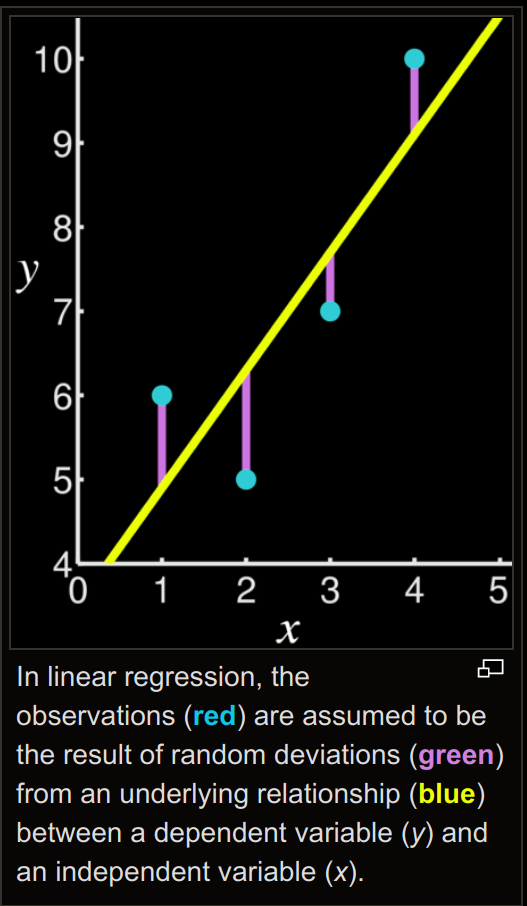
\includegraphics[scale=0.2]{Linear_Regression-neg.png}
\vfill
Goal: Find a blue line that minimizes \\
the sum of the square of the green lines
\end{frame}
%-------------- end slide -------------------------------%}}}
%-------------- start slide -------------------------------%{{{ 11.19
\begin{frame}
\begin{enumerate}
\item[Thm.~] Given $n$ points $(x_1,y_1),\cdots, (x_n,y_n)$, the straight line $y=a+bx$ minimizing \[
		L(a,b) = \sum_{i=1}^n \left[y_i-(a+bx_i) \right]^2
\]
when
\[
b= \frac{n\sum_{i=1}^n x_iy_i - \left(\sum_{i=1}^n x_i\right)\left(\sum_{i=1}^n y_i\right)}{n\left(\sum_{i=1}^n x_i^2\right)-\left(\sum_{i=1}^n x_i\right)^2}
\]
and
\[
a =  \frac{\sum_{i=1}^ny_i-b\sum_{i=1}^nx_i}{n} = \bar y - b \bar x.
\]
\vfill
\item[Proof.]
\begin{align}
\tag{Normal equations}
\begin{cases}
\displaystyle
\frac{\partial }{\partial a}L(a,b) = \sum_{i=1}^n (-2) \left[y_i-(a+bx_i) \right] = 0\\
\displaystyle
\frac{\partial }{\partial b} L(a,b) = \sum_{i=1}^n (-2x_i) \left[y_i-(a+bx_i) \right] = 0\\
\end{cases}
\end{align}
\end{enumerate}
\end{frame}
%-------------- end slide -------------------------------%}}}
%-------------- start slide -------------------------------%{{{ 11.20
\begin{frame}[fragile]
	\[
		\Longleftrightarrow\qquad
\begin{cases}
\displaystyle
\sum_{i=1}^n y_i-n a- b \sum_{i=1}^n x_i = 0& \hspace{5em} (1)\\[1em]
\displaystyle
\sum_{i=1}^n x_iy_i - a \sum_{i=1}^n x_i - b\sum_{i=1}^n x_i^2 =0&\hspace{5em} (2)
\end{cases}
	\]
	\vfill
	\begin{align*}
		(1) & \quad\Longrightarrow \quad a = \bar{y}-b\bar{x}\\[2em]
		(1)\times \sum_{i=1}^n x_i - (2)\times n &\quad\Longrightarrow\quad
	b= \frac{n\sum_{i=1}^n x_iy_i - \left(\sum_{i=1}^n x_i\right)\left(\sum_{i=1}^n y_i\right)}{n\left(\sum_{i=1}^n x_i^2\right)-\left(\sum_{i=1}^n x_i\right)^2}
	\end{align*}
\myEnd
\end{frame}
%-------------- end slide -------------------------------%}}}
%-------------- start slide -------------------------------%{{{ 11.21
\begin{frame}{(Moore-Penrose) Pseudoinverse}

	\begin{enumerate}
		\item Well determined system
			\[
				Ax = b \quad\Longrightarrow\quad x = A^{-1} y.
			\]
			\vfill
		\item Overdetermined system
			\begin{align*}
				Ax &= y\\
				A^T A x &= A^T y \\
				\underbrace{(A^T A)^{-1}A^T A}_{=I} x &= (A^T A)^{-1}A^T y \\
				x &= \underbrace{(A^T A)^{-1}A^T}_{=: A^+} y \\
			\end{align*}
			\vfill
		\item Under determined system
			\[
				Ax= y \quad\Longrightarrow\quad x = \underbrace{A^T(AA^T)^{-1}}_{=:A^+} y.
			\]
	\end{enumerate}
\end{frame}
%-------------- end slide -------------------------------%}}}
%-------------- start slide -------------------------------%{{{ 11.22
\begin{frame}[fragile]

	\begin{enumerate}
		\item[Proof.] (Another proof based on pseudoinverse)
	\[
A =
\begin{pmatrix}
	1 & x_1\cr
	1 & x_2 \cr
	\vdots & \vdots \cr
	1 & x_n
\end{pmatrix}_{n\times 2}, \qquad
x =
\begin{pmatrix}
	\beta_0\cr
	\beta_1
\end{pmatrix}_{2\times 1},\qquad
y =
\begin{pmatrix}
	y_1\cr
	y_2\cr
	\vdots\cr
	y_n\cr
\end{pmatrix}_{1\times n}
	\]
	\vfill
\item[]
	\[
	A^T A =
	\begin{pmatrix}
		1 & 1 & \cdots & 1\cr
		x_1 & x_2 & \cdots & x_n \cr
\end{pmatrix}\begin{pmatrix}
	1 & x_1\cr
	1 & x_2 \cr
	\vdots & \vdots \cr
	1 & x_n
\end{pmatrix}
=
\begin{pmatrix}
	n & \sum_{i=1}^n x_i\cr
	\sum_{i=1}^n x_i & \sum_{i=1}^n x_i^2
\end{pmatrix}
	\]
\vfill
\item[]
\[
	(A^TA)^{-1}  =
% \begin{pmatrix}
	% n & \sum_{i=1}^n x_i\cr
	% \sum_{i=1}^n x_i & \sum_{i=1}^n x_i^2
% \end{pmatrix}^{-1}=
\frac{1}{n\sum_{i=1}^n x_i^2-\left(\sum_{i=1}^n x_i\right)^2}
\begin{pmatrix}
	\sum_{i=1}^n x_i^2
 & -\sum_{i=1}^n x_i\cr
	-\sum_{i=1}^n x_i & n \end{pmatrix}
\]
\end{enumerate}
\end{frame}
%-------------- end slide -------------------------------%}}}
%-------------- start slide -------------------------------%{{{ 11.23
\begin{frame}[fragile]

	\begin{enumerate}
		\item[]
	\[
	A^T y =	\begin{pmatrix}
		1 & 1 & \cdots & 1\cr
		x_1 & x_2 & \cdots & x_n \cr
\end{pmatrix}
\begin{pmatrix}
	y_1\cr
	y_2\cr
	\vdots\cr
	y_n\cr
\end{pmatrix} =
\begin{pmatrix}
	\sum_{i=1}^n y_i \cr
	\sum_{i=1}^n x_iy_i \cr
\end{pmatrix}
	\]
	\vfill
\item[]
	\begin{align*}
		\begin{pmatrix}
			a\cr
			b\cr
		\end{pmatrix}=
x =&
(A^TA)^{-1}A^T y\\[1em]
		=&
\frac{1}{n\sum_{i=1}^n x_i^2-\left(\sum_{i=1}^n x_i\right)^2}
\begin{pmatrix}
	\sum_{i=1}^n x_i^2
 & -\sum_{i=1}^n x_i\cr
	-\sum_{i=1}^n x_i & n
\end{pmatrix}
\begin{pmatrix}
	\sum_{i=1}^n y_i \cr
	\sum_{i=1}^n x_iy_i \cr
\end{pmatrix}\\[3em]
		 =&
		 \begin{pmatrix}
			 \displaystyle
			 \frac{\left(\sum_{i=1}^n x_i^2\right)\left( \sum_{i=1}^n y_i\right) - \left(\sum_{i=1}^n x_i\right)\left(\sum_{i=1}^n x_iy_i\right)}{n\sum_{i=1}^n x_i^2-\left(\sum_{i=1}^n x_i\right)^2} \\[2em]
			 \displaystyle
\frac{n\sum_{i=1}^n x_iy_i - \left(\sum_{i=1}^n x_i\right)\left(\sum_{i=1}^n y_i\right)}{n\sum_{i=1}^n x_i^2-\left(\sum_{i=1}^n x_i\right)^2} \cr
		 \end{pmatrix}
	\end{align*}
	\end{enumerate}
\end{frame}
%-------------- end slide -------------------------------%}}}
%-------------- start slide -------------------------------%{{{ 11.24
\begin{frame}[fragile]
	\[
	b =
\frac{n\sum_{i=1}^n x_iy_i - \left(\sum_{i=1}^n x_i\right)\left(\sum_{i=1}^n y_i\right)}{n\sum_{i=1}^n x_i^2-\left(\sum_{i=1}^n x_i\right)^2}.
	\]
	\vfill
	\begin{align*}
		a=&
			 \frac{\left(\sum_{i=1}^n x_i^2\right)\left( \sum_{i=1}^n y_i\right) - \left(\sum_{i=1}^n x_i\right)\left(\sum_{i=1}^n x_iy_i\right)}{n\sum_{i=1}^n x_i^2-\left(\sum_{i=1}^n x_i\right)^2} \\[2em]
			 =&		 \frac{\left(\sum_{i=1}^n x_i^2\right)\left( \sum_{i=1}^n y_i\right) - \left(\sum_{i=1}^n x_i\right)\left[\left(\sum_{i=1}^n x_iy_i\right)-\frac 1n \left(\sum_{i=1}^n x_i\right)\left(\sum_{i=1}^n y_i\right)\right]}{n\sum_{i=1}^n x_i^2-\left(\sum_{i=1}^n x_i\right)^2} \\[2em]
			 &-  \frac{\frac 1n \left(\sum_{i=1}^n x_i\right)^2\left(\sum_{i=1}^n y_i\right)}{n\sum_{i=1}^n x_i^2-\left(\sum_{i=1}^n x_i\right)^2}\\[2em]
			 =&
			 \frac 1n \sum_{i=1}^n y_i - b\frac{1}{n} \sum_{i=1}^nx_i
			 = \bar{y} -b \bar{x}.
	\end{align*}
	\myEnd
\end{frame}
%-------------- end slide -------------------------------%}}}
%-------------- start slide -------------------------------%{{{ 11.25
\begin{frame}[fragile]{A probabilistic view ... }
\begin{enumerate}
\item[Def.] The function $f(X)$ for which
\[
\E\left[  \left(Y-f(X)\right)^2\right]
\]
is minimized is called the \textcolor{yellow!80!black}{\bf regression curve of $Y$ on $X$}.
\vfill
\item[Thm.] Let $(X,Y)$ be two random variables such that $\Var(X)$ and $\Var(Y)$ both exist.
Then the regression cure of $Y$ on $X$ is given (for all $x$) by
\[
f(x) = \E \left[Y|X=x \right].
\]
\end{enumerate}
\end{frame}
%-------------- end slide -------------------------------%}}}
%-------------- start slide -------------------------------%{{{ 11.26
\begin{frame}
\begin{enumerate}
\item[Proof.] Let $f(x)= \E \left[Y|X=x \right]$ and let $\phi(x)$ be a general function. Then
\begin{align*}
	\E\left[  \left(Y-\phi(X)\right)^2\right]= & \E\left[ \left([Y-f(X)]+ [f(X)-\phi(X)]\right)^2\right]                             \\
	                                         = & \E\left[ \left(Y-f(X)\right)^2\right] +\E\left[  \left(f(X)-\phi(X)\right)^2\right] \\
                                             & +\E\left[ \left(Y-f(X)\right) \left(f(X)-\phi(X)\right)\right].
\end{align*}
\item[] Let $\psi(x)$ be either $f(x)$ or $\phi(x)$. We claim that
\begin{align*}
\E\left[  \left(Y-f(X)\right) \psi(X)\right] =0.
\end{align*}
\item[] Indeed,
\begin{align*}
	\E[Y\psi(X)] & = \iint_{\R^2} f_{X,Y}(x,y)y\psi(x)\ud y\ud x \\
							 & = \int_\R \ud x \psi(x) f_X(x) \underbrace{\int_\R \ud y  \frac{f_{X,Y}(x,y)}{f_X(x)} y}_{\displaystyle = \E[Y|X=x] }\\
							 & = \E[f(X)\psi(X)].
\end{align*}
\item[] Hence,
\[
\E\left[  \left(Y-\phi(X)\right)^2\right]=
\E\left[  \left(Y-f(X)\right)^2\right] +\E\left[  \left(f(X)-\phi(X)\right)^2\right]
\]
which is minimized when $\phi(x)=f(x)$.\myEnd
\end{enumerate}
\end{frame}
%-------------- end slide -------------------------------%}}}
%-------------- start slide -------------------------------%{{{ 11.27
\begin{frame}[fragile]

	\begin{enumerate}
		\item[] If one imposes that $f(x) = a+bx$, then
			\vfill
		\item[Thm.] The following squared error:
			\[
				\E\left[ \left\{ Y - \left( a+b X\right )\right\}^2  \right ]
			\]
		\item[] is minimized at
			\[
				b = \rho_{XY}\frac{\sigma_Y}{\sigma_X}=  \frac{\sigma_{XY}}{\sigma_X^2} \quad
				\text{and}\quad
				a = \E[Y] -b \E[X]
			\]
		\item[] with the mean squared error
			\[
				\E\left[ \left\{ Y - \left( a+b X\right )\right\}^2  \right ] = \left(1-\rho_{XY}^2 \right )\sigma_Y^2.
			\]
	\end{enumerate}
\end{frame}
%-------------- end slide -------------------------------%}}}
%-------------- start slide -------------------------------%{{{ 11.28
\begin{frame}[fragile]

\begin{enumerate}
\item[Proof.]
\begin{align*}
&\E\left[ \left\{ Y - \left( a+b X\right )\right\}^2  \right ]\\
=&
\E\left[ \bigg\{ [Y-\E(Y)] - b[X-\E(X)] - \left[ a-\E[Y] +b \E(X)\right ]\bigg\}^2  \right ]
\end{align*}
\item[]
\begin{minipage}{0.5\textwidth}
	\begin{gather*}
	||\\
\E\left[ \left[Y-\E(Y)\right]^2  \right ]\\
+
b^2 \E\left[ \left[X-\E(X)\right]^2 \right]\\
+ \bigg[ a-\E[Y] +b \E(X)\bigg]^2\\
-2b
\E\bigg[ [Y-\E(Y)] [X-\E(X)] \bigg]\\
-2\bigg[ a-\E[Y] +b \E(X)\bigg] \E\left[ Y-\E(Y)\right]\\
+2b\bigg[ a-\E[Y] +b \E(X)\bigg] \E\left[ X-\E(X)\right]
	\end{gather*}
\end{minipage}
\pause \hfill =\hfill
\begin{minipage}{0.3\textwidth}
	\begin{gather*}
		\Var(Y) \\[0.7em]
		+b^2 \Var(X)\\[0.7em]
		+ \bigg[ a-\E[Y] +b \E(X)\bigg]^2\\[1em]
		-2b\: \Cov(X,Y)\\[1.1em]
		+ 0 \\[1.1em]
+0
	\end{gather*}
\end{minipage}
\end{enumerate}
\end{frame}
%-------------- end slide -------------------------------%}}}
%-------------- start slide -------------------------------%{{{ 11.29
\begin{frame}[fragile]

	\begin{enumerate}
		\item[]
	\begin{gather*}
		\Downarrow\\
\E\left[ \left\{ Y - \left( a+b X\right )\right\}^2  \right ]\\
|| \\
		 \Var(Y)
		+b^2 \Var(X)
		+ \bigg[ a-\E[Y] +b \E(X)\bigg]^2
		-2b\: \Cov(X,Y)
	\end{gather*}
	\vfill
\item[] The best $a$, called $a^*$, should be such that
	\vfill
	\[
		 \bigg[ a^*-\E[Y] +b \E(X)\bigg]^2 = 0
		 \quad\Longleftrightarrow\quad
		 a^* = \E[Y]-b\E[X]
	\]
	\end{enumerate}
\end{frame}
%-------------- end slide -------------------------------%}}}
%-------------- start slide -------------------------------%{{{ 11.30
\begin{frame}[fragile]

\begin{enumerate}
	\item[]
	\begin{gather*}
		\Downarrow\\
\E\left[ \left\{ Y - \left( a^*+b X\right )\right\}^2  \right ]\\
|| \\
		 \Var(Y)
		+b^2 \Var(X)
		-2b\: \Cov(X,Y)\\
		|| \\
		\sigma_Y^2 + b^2 \sigma_X^2 -2b\rho_{XY}\sigma_X\sigma_Y\\
		||\\
		\left(1-\rho_{XY}^2\right)\sigma_Y^2 +
		\bigg(b\sigma_X -\rho_{XY}\sigma_Y \bigg)^2
	\end{gather*}
	\vfill
\item[] The best $b$, called $b^*$, should be
	\vfill
	\[
		\left(b^*\sigma_X -\rho_{XY}\sigma_Y \right)^2 =0
		\quad\Longleftrightarrow\quad
		b^* = \rho_{XY}\frac{\sigma_Y}{\sigma_X}
	\]
\end{enumerate}
\end{frame}
%-------------- end slide -------------------------------%}}}
%-------------- start slide -------------------------------%{{{ 11.31
\begin{frame}[fragile]

	\begin{enumerate}
		\item[]
	\begin{gather*}
		\Downarrow\\
\E\left[ \left\{ Y - \left( a^*+b^* X\right )\right\}^2  \right ]\\
|| \\
\left(1-\rho_{XY}^2\right)\sigma_Y^2
	\end{gather*}
	\vfill
\item[] with
	\vfill
			\[
				b^* = \rho_{XY}\frac{\sigma_Y}{\sigma_X}=  \frac{\sigma_{XY}}{\sigma_X^2} \qquad
				\text{and}\qquad
				a^* = \E[Y] -b \E[X]
			\]
			\myEnd
	\end{enumerate}
\end{frame}
%-------------- end slide -------------------------------%}}}
%-------------- start slide -------------------------------%{{{ 11.32
\begin{frame}[fragile]

\begin{enumerate}
\item[Remark] In practice, we have data $(x_1,y_1),\cdots,(x_n,y_n)$ instead of the joint law of $(X,Y)$ \\
\[\Downarrow\]
\begin{center}
Replace\\[1em]
$\mu_X, \mu_Y, \sigma_X^2,\sigma_Y^2,\rho_{XY}, \sigma_{XY}$
\\[1em]
by their maximum likelihood estimates\\[1em]
$\bar{x},\bar{y},\hat{\sigma}_X^2,\hat{\sigma}_Y^2,r_{XY},\hat{\sigma}_{XY}$
\end{center}
\end{enumerate}
\end{frame}
%-------------- end slide -------------------------------%}}}
%-------------- start slide -------------------------------%{{{ 11.33
\begin{frame}
\begin{enumerate}
\item $\bar x = \frac{1}{n}\sum_{i=1}^n x_i$, $\bar y = \frac{1}{n}\sum_{i=1}^n y_i$\\[2em]
\item $\displaystyle \hat{\sigma}_X^2 =  \frac{1}{n}\sum_{i=1}^n \left(x_i-\bar x \right)^2= \frac{1}{n}\sum_{i=1}^n x_i^2 -\bar x^2=  \frac{n\sum_{i=1}^n x_i^2 - \left(\sum_{i=1}^n x_i \right)^2}{n^2}$
\item[]  $\displaystyle \hat{\sigma}_Y^2 =  \frac{1}{n}\sum_{i=1}^n \left(y_i-\bar y \right)^2= \frac{1}{n}\sum_{i=1}^n y_i^2 -\bar y^2=  \frac{n\sum_{i=1}^n y_i^2 - \left(\sum_{i=1}^n y_i \right)^2}{n^2}$ \\[2em]
\item $\displaystyle \hat{\sigma}_{XY}= \frac{1}{n}\sum_{i=1}^n \left(x_i-\bar x \right)\left(y_i-\bar y \right)=
	\frac{1}{n}\sum_{i=1}^n x_iy_i - \bar{x}\bar{y} $\\[0.5em]
	\hspace{2em}$\displaystyle =  \frac{n\sum_{i=1}^n x_iy_i -
		\left(\sum_{i=1}^n x_i \right)
		\left(\sum_{i=1}^n y_i \right)
	}{n^2}$\\[2em]
\item $\displaystyle r_{XY} =  \frac{\hat{\sigma}_{XY}}{\hat{\sigma}_X \hat{\sigma}_Y}$
\item[]
	\[
	\Downarrow
	\]
	\[
		\boxed{b = r_{XY} \frac{\hat{\sigma}_Y}{\hat{\sigma}_X} = \frac{\hat{\sigma}_{XY}}{\hat{\sigma}_X^2},
		\qquad a = \bar{y}-b\bar{x}}
	\]
\end{enumerate}
\end{frame}
%-------------- end slide -------------------------------%}}}
%-------------- start slide -------------------------------%{{{ 11.34
\begin{frame}[fragile]
	\begin{minipage}{0.45\textwidth}
		\begin{center}
			Maximum likelihood estimates
			\[ \hat{\sigma}_X^2 =  \frac{1}{n}\sum_{i=1}^n \left(x_i-\bar x \right)^2
			\]
			\[
			 \hat{\sigma}_Y^2 =  \frac{1}{n}\sum_{i=1}^n \left(y_i-\bar y \right)^2
			 \]\[
		 \hat{\sigma}_{XY}= \frac{1}{n}\sum_{i=1}^n \left(x_i-\bar x \right)\left(y_i-\bar y \right)
		 \]
		\end{center}
	\end{minipage}
	\hfill
	\begin{minipage}{0.45\textwidth}
		\begin{center}
			Sample (co)variances
			\[ s_X^2 =  \frac{1}{n-1}\sum_{i=1}^n \left(x_i-\bar x \right)^2
			\]
			\[
			 s_Y^2 =  \frac{1}{n-1}\sum_{i=1}^n \left(y_i-\bar y \right)^2
			 \]\[
		 s_{XY}= \frac{1}{n-1}\sum_{i=1}^n \left(x_i-\bar x \right)\left(y_i-\bar y \right)
		 \]
		\end{center}
	\end{minipage}
\end{frame}
%-------------- end slide -------------------------------%}}}
%-------------- start slide -------------------------------%{{{ 11.35
\begin{frame}
\begin{enumerate}
\item[E.g. 1] Producing air conditioners. $x=$ rough weight of a rod. $y=$ finished weight.
Find the best linear approximation of $xy$-relationship.
Predict the weight when $x=2.71$
\\[1em]
\begin{center}
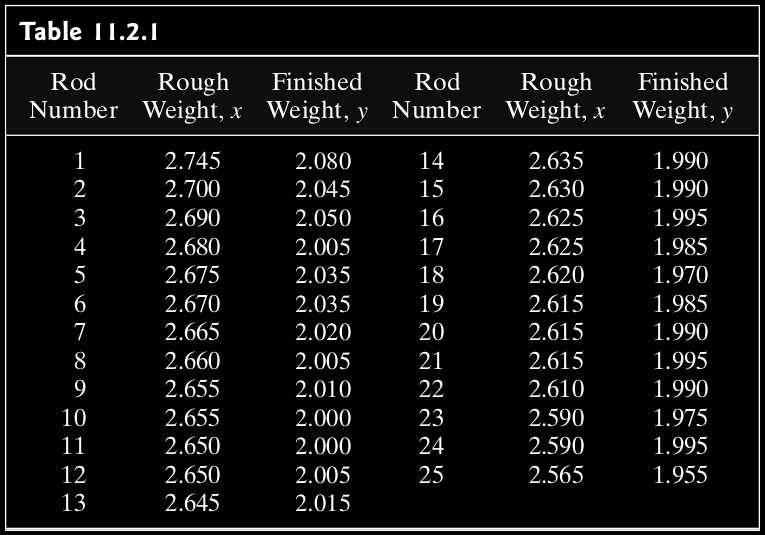
\includegraphics[scale=0.25]{Table_11-2-1-neg.png}
\end{center}
\end{enumerate}
\end{frame}
%-------------- end slide -------------------------------%}}}
%-------------- start slide -------------------------------%{{{ 11.36
\begin{frame}

\begin{enumerate}
\item[Sol.] ...\\[1em]
\vfill
\begin{center}
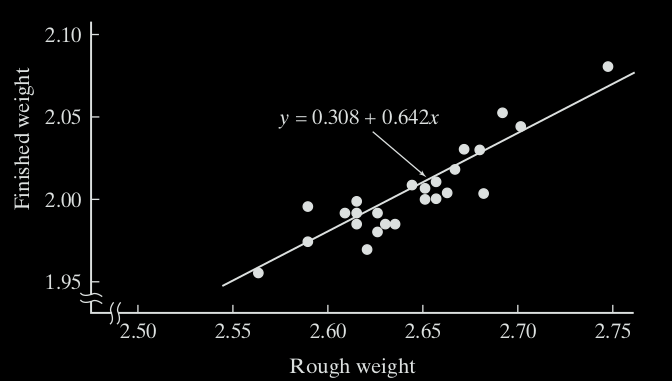
\includegraphics[scale=0.25]{Figure_11-2-1-neg.png}
\end{center}
\vfill
... \myEnd
\end{enumerate}
\end{frame}
%-------------- end slide -------------------------------%}}}
%-------------- start slide -------------------------------%{{{ 11.37
\begin{frame}

\begin{enumerate}
\item[Def.] Let $a$ and $b$ be the least squares coefficients with the sample $(x_1,y_1),\cdots, (x_n,y_n)$.
\\[1em]
\item[] $\hat y=a+bx$: {\bf \textcolor{yellow}{predicted value}} of y
\\[1em]
\item[] $y_i-\hat y_i = y_i - (a+bx_i)$: {\bf \textcolor{yellow}{$i$th residual}}
\vfill
\item[Remark] Use the residual plots to assessing the model.
\end{enumerate}
\end{frame}
%-------------- end slide -------------------------------%}}}
%-------------- start slide -------------------------------%{{{ 11.38
\begin{frame}

\begin{enumerate}
\item[E.g. 1'] Here are the residues and their plots:\\[1em]
\vfill
\begin{minipage}{0.43\textwidth}
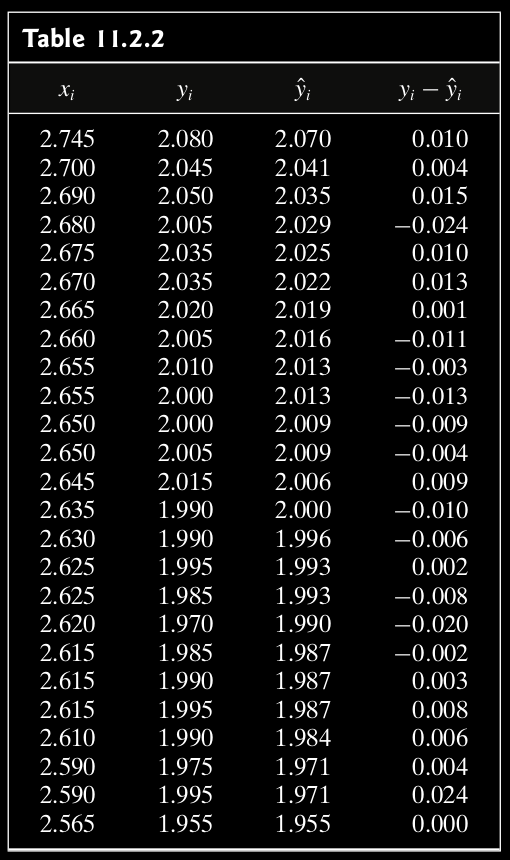
\includegraphics[scale=0.15]{Table_11-2-2-neg.png}
\end{minipage}
\begin{minipage}{0.5\textwidth}
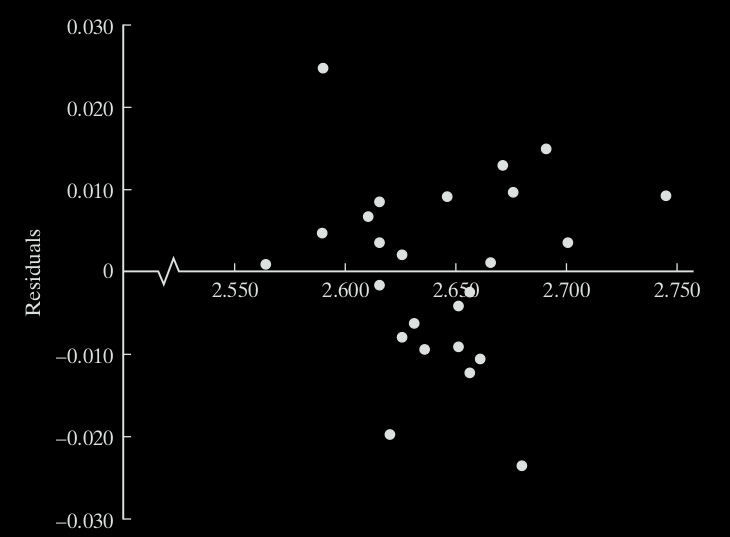
\includegraphics[scale=0.2]{Figure_11-2-2-neg.png}
\end{minipage}
\end{enumerate}

\end{frame}
%-------------- end slide -------------------------------%}}}
%-------------- start slide -------------------------------%{{{ 11.39
\begin{frame}

\begin{enumerate}
\item[E.g. 2] Predict the Social Security expenditures.
\begin{center}
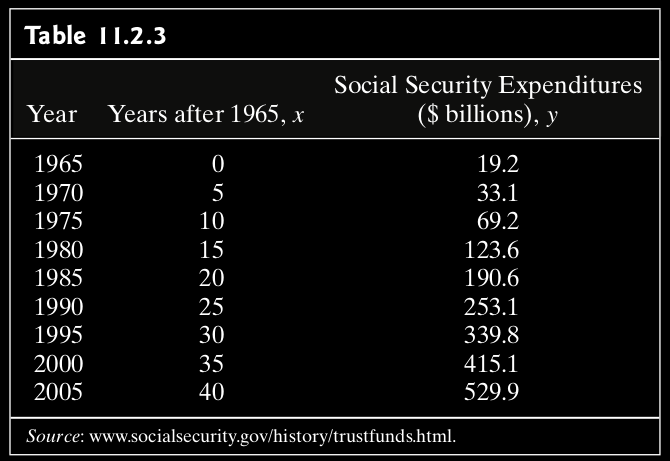
\includegraphics[scale=0.25]{Table_11-2-3-neg.png}
\end{center}
Does the the least squares line $y=-38.0+12.9x$ a good model to predict the cost in 2010 would be $\$543$, i.e., the case $x=45$?
\vfill
\item[Sol.]
\end{enumerate}
\end{frame}
%-------------- end slide -------------------------------%}}}
%-------------- start slide -------------------------------%{{{ 11.40
\begin{frame}
\centering
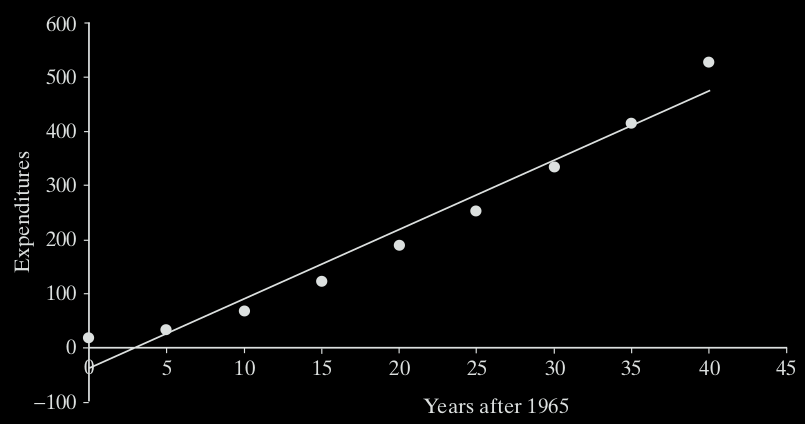
\includegraphics[scale=0.25]{Figure_11-2-3-neg.png}
\\
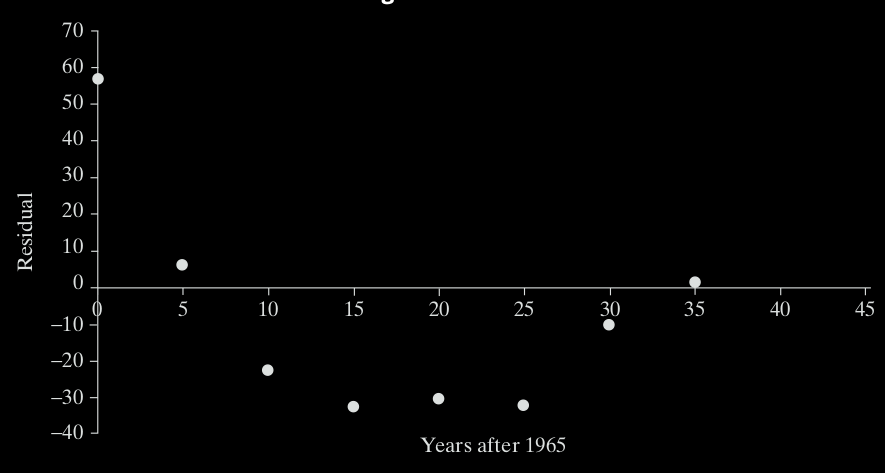
\includegraphics[scale=0.25]{Figure_11-2-4-neg.png}
\end{frame}
%-------------- end slide -------------------------------%}}}
%-------------- start slide -------------------------------%{{{ 11.41
\begin{frame}
	\centering
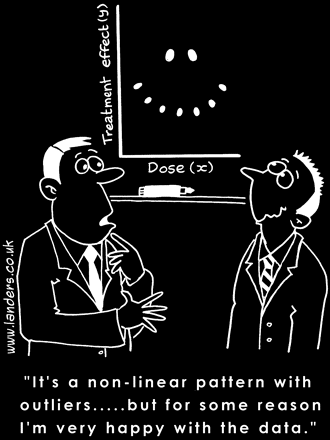
\includegraphics[scale=0.5]{Nonlinear_regression-neg.png}
\end{frame}
%-------------- end slide -------------------------------%}}}
%-------------- start slide -------------------------------%{{{ 11.42
\begin{frame}{Exponential Regression}
\centering
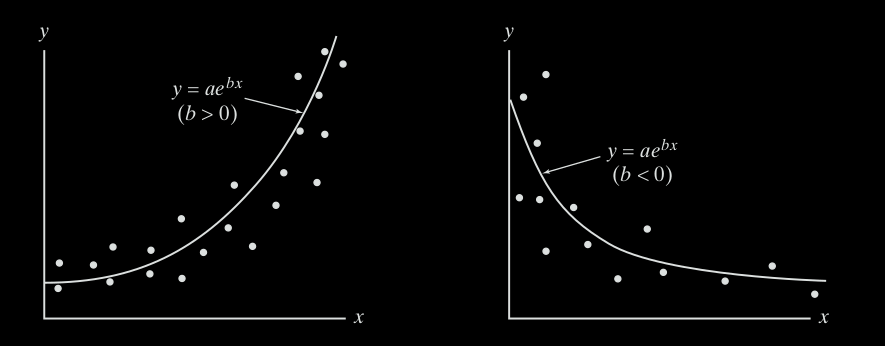
\includegraphics[scale=0.25]{Figure_11-2-7-neg.png}
\vfill
\[
y=a e^{bx} \quad \Longleftrightarrow \quad \ln y = \ln a + b x
\]
\vfill
\[
b= \frac{n\sum_{i=1}^n x_i\alert{\ln y_i} - \left(\sum_{i=1}^n x_i\right)\left(\sum_{i=1}^n \alert{\ln y_i}\right)}{n\left(\sum_{i=1}^n x_i^2\right)-\left(\sum_{i=1}^n x_i\right)^2}
\qquad
\alert{\ln a} =  \frac{\sum_{i=1}^n\alert{\ln y_i}-b\sum_{i=1}^nx_i}{n}
\]
\end{frame}
%-------------- end slide -------------------------------%}}}
%-------------- start slide -------------------------------%{{{ 11.43
\begin{frame}

\begin{enumerate}
\item[E.g.] Moore's law: \\[1em]
Gordon Moore predicted in 1965 that the number of transistors per chip would double every 18 months. \\[1em]
\item[] Based on the real data, check:
\item[] 1) Whether is the chip capacity doubling at a fixed rate?
\item[] 2) Find out the rate.
\vfill
\begin{center}
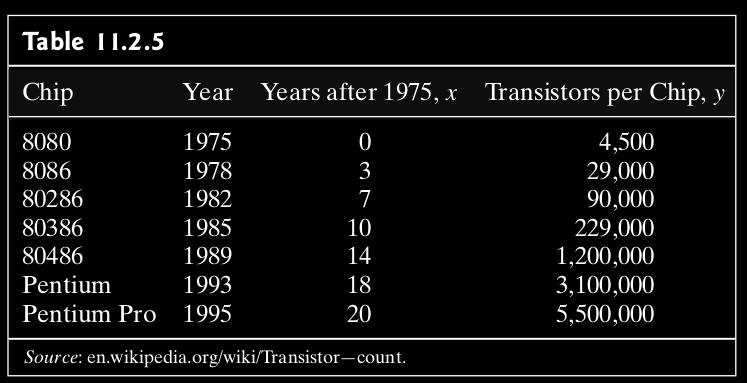
\includegraphics[scale=0.25]{Table_11-2-5-neg.png}
\end{center}
\end{enumerate}
\end{frame}
%-------------- end slide -------------------------------%}}}
%-------------- start slide -------------------------------%{{{ 11.44
\begin{frame}

\begin{enumerate}
\item[Sol.] To check whether chip capacity doubles in a fixed rate, one needs to
carry out exponential regression:
\vfill
\begin{center}
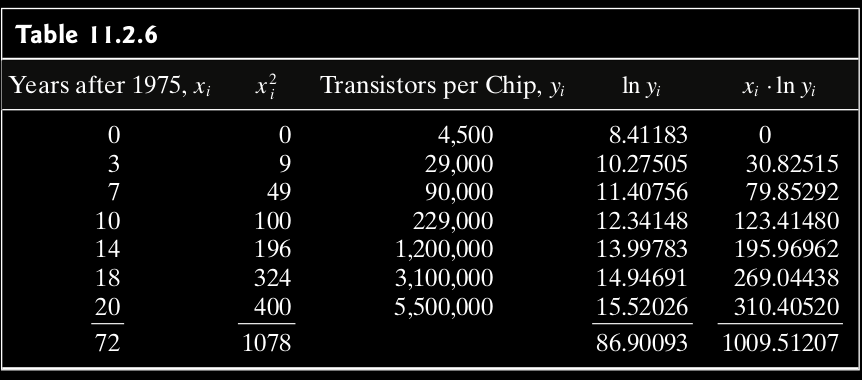
\includegraphics[scale=0.2]{Table_11-2-6-neg.png}
\vfill
\[
\Longrightarrow\quad	b = \cdots = 0.342810, \quad a = \cdots = e^{\ln a} = e^{8.89} = 7247.189.
\]
\vfill
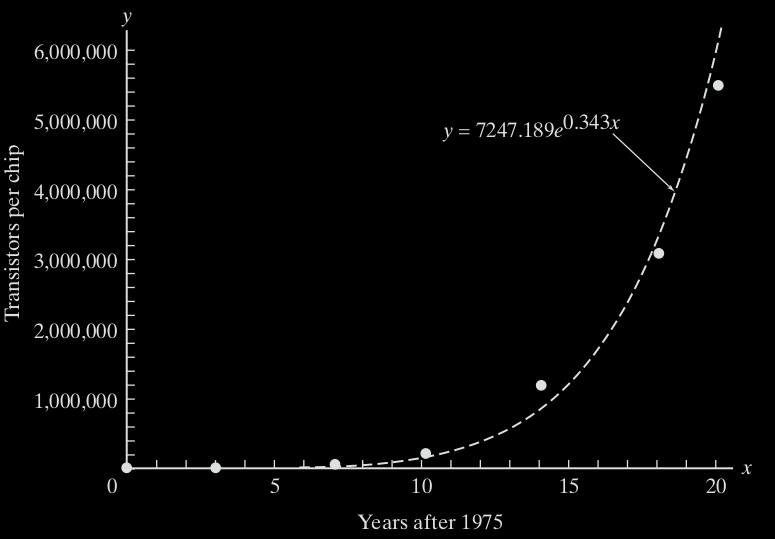
\includegraphics[scale=0.2]{Figure_11-2-8-neg.png}
\end{center}
\end{enumerate}
\end{frame}
%-------------- end slide -------------------------------%}}}
%-------------- start slide -------------------------------%{{{ 11.45
\begin{frame}

\begin{enumerate}
\item[] Finally, to find out the rate:
\vfill
\[
e^{0.343 x} = e^{\ln 2 \times  \frac{0.343}{\ln 2} x} = 2^{ \frac{0.343}{\ln 2}x}
\]
\vfill
\[
\frac{0.343}{\ln 2} x = 1 \quad \Longrightarrow \quad x =  \frac{\ln 2}{0.343} = 2.020837.
\]
\myEnd

\end{enumerate}
\end{frame}
%-------------- end slide -------------------------------%}}}
%-------------- start slide -------------------------------%{{{ 11.46
\begin{frame}{Other curvilinear models}
\centering
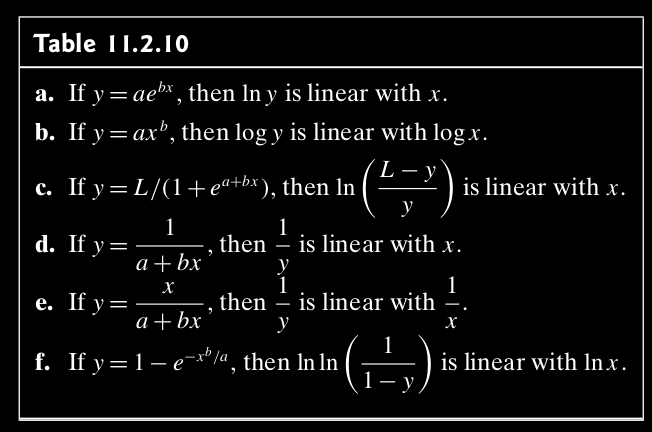
\includegraphics[scale=0.3]{Table_11-2-10-neg.png}
\end{frame}
%-------------- end slide -------------------------------%}}}

\mySection{11.3 The Linear Model}
%-------------- start slide -------------------------------%{{{ 10.49
\begin{frame}
	% {\S\: 11.3 The Linear Model}
	\phantom{a}\hfill
	\begin{minipage}{0.95\textwidth}
\begin{enumerate}[leftmargin=15em]
\item[Recall] For any two random variables $X$ and $Y$, the regression curve of $Y$ on $X$, namely,
\[
f(x) = \E \left[Y|X=x \right].
\]
minimizes the squared error
\[
\E\left[  \left(Y-f(X)\right)^2\right]
\]
\vspace{3em}
\item[Difficulties] The regression curve $y=\E[Y|x]$ is complicated and hard to obtain.
\vspace{3em}
\item[Compromise] Assume that $f(x)=a+bx$ \quad (i.e., the first order approximation)
\end{enumerate}
	\end{minipage}
\end{frame}
%-------------- end slide -------------------------------%}}}
%-------------- start slide -------------------------------%{{{ 10.50
\begin{frame}
\begin{enumerate}
	\item[Def.] \textcolor{yellow!80!black}{\bf (Simple) linear model}:
	\item[] 1. $f_{Y|x}(y)$ is a normal pdf for any $x$ given.
	\vfill
	\item[] 2. The standard deviation, $\sigma$, of $Y|x$ is the same for all $x$, i.e.,
	\[
	\sigma^2 \equiv \E[Y^2|x] - \E[Y|x]^2.
	\]
	\vfill
	\item[] 3. The mean of $Y|x$ is collinear, i.e.,
	\[
	y = \E[Y|x] = \beta_0 + \beta_1 x.
	\]
	\item[] 4. All of the conditional distributions represnt indep. random variables.
		\vfill
	\item[Summary] Let $Y_1,\cdots,Y_n$ be independent r.v.'s where $Y_i\sim N(\beta_0+\beta_1x_i,\sigma^2)$ with $x_i$ are known and $\beta_0$, $\beta_1$ and $\sigma^2$ are unknown.
		\[\text{\rotatebox[origin=c]{90}{$\Leftrightarrow$}}\]
		\[
			Y_i = \beta_0+\beta_1 x_i + \epsilon_i, \quad \text{$\epsilon_i$ are indep. and $\epsilon_i\sim N(0,\sigma^2)$}.
		\]
\end{enumerate}
\end{frame}
%-------------- end slide -------------------------------%}}}
%-------------- start slide -------------------------------%{{{ 10.51
\begin{frame}
\centering
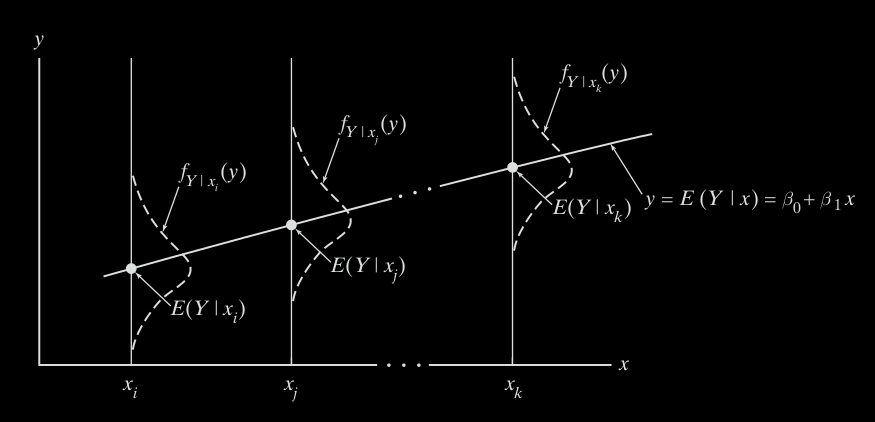
\includegraphics[scale=0.35]{Figure_11-3-2-neg.png}
\end{frame}
%-------------- end slide -------------------------------%}}}
%-------------- start slide -------------------------------%{{{ 10.52
\begin{frame}{MLE for linear model}

\begin{enumerate}
	\item[Thm.] Let $(x_1,Y_1),\cdots, (x_n,Y_n)$ be a set of points satisfying the linear model, $\E[Y|x]=\beta_0+\beta_1 x$.
		\bigskip
	\item[] ($\Longleftrightarrow$
		let $Y_1,\cdots,Y_n$ be independent r.v.'s where $Y_i\sim N(\beta_0+\beta_1x_i,\sigma^2)$ with $x_i$ are known and $\beta_0$, $\beta_1$ and $\sigma^2$ are unknown.)
		\bigskip
\item[]	The maximum likelihood estimators for $\beta_0$, $\beta_1$ and $\sigma^2$ are given by
	\vfill
\[
\hat\beta_1= \frac{n\sum_{i=1}^n x_iY_i - \left(\sum_{i=1}^n x_i\right)\left(\sum_{i=1}^n Y_i\right)}{n\left(\sum_{i=1}^n x_i^2\right)-\left(\sum_{i=1}^n x_i\right)^2}
\]
\bigskip
\[
\hat\beta_0 =  \frac{\sum_{i=1}^nY_i-\hat{\beta_1}\sum_{i=1}^nx_i}{n} = \overline{Y} - \hat\beta_1 \overline{x}
\]
\medskip
\[
\hat\sigma^2 =  \frac{1}{n}\sum_{i=1}^{n} \left(Y_i-\widehat Y_i \right)^2,\qquad \widehat Y_i = \hat\beta_0 + \hat\beta_1 x_i.
\]
\end{enumerate}
\end{frame}
%-------------- end slide -------------------------------%}}}
%-------------- start slide -------------------------------%{{{ 1. Proof of the Theorem 1/4
\begin{frame}[fragile]
\begin{itemize}
	\item[Proof.] Since $Y_i\sim N\left(\beta_0+\beta_1x_i,\sigma^2\right)$,
	\begin{align*}
		L(\beta_0,\beta_1,\sigma^2) = \prod_{i=1}^n f_{Y_i|x_i}(y_i) = \prod_{i=1}^n \frac{1}{\sqrt{2\pi\sigma^2}} \exp\left(-\frac{(y_i-\beta_0-\beta_1x_i)^2}{2\sigma^2}\right).
	\end{align*}
	\item[] Then take partial derivatives and set them to zero:
	\begin{align*}
		\frac{\partial\ln L}{\partial \beta_0} & = \frac{1}{\sigma^2} \sum_{i=1}^n (y_i-\beta_0-\beta_1 x_i) = 0\\
		\frac{\partial\ln L}{\partial \beta_1} & = \frac{1}{\sigma^2} \sum_{i=1}^n (y_i-\beta_0-\beta_1 x_i) x_i = 0\\
		\frac{\partial\ln L}{\partial \sigma^2} & = -\frac{n}{2\sigma^2} + \frac{1}{(\sigma^2)^2} \sum_{i=1}^n (y_i-\beta_0-\beta_1 x_i)^2 =0
	\end{align*}
	\end{itemize}
\end{frame}
%-------------- end slide -------------------------------%}}}
%-------------- start slide -------------------------------%{{{ 1. Proof of the Theorem 2/4
\begin{frame}[fragile]
\begin{itemize}
	\item[] Once $\beta_0$  and $\beta_1$ are solved from the first relations, then the third relation shows that
	\begin{align*}
		\sigma^2 = \frac{1}{n} \sum_{i=1}^n (y_i-\beta_0-\beta_1x_i)^2.
	\end{align*}
	\item[] The first two relations give
	\begin{align*}
		& \left(\sum_{i=1}^n y_i\right) - \beta_0  n - \beta_1 \left(\sum_{i=1}^n x_i\right) = 0\\
		& \left(\sum_{i=1}^n x_iy_i\right) - \beta_0 \left(\sum_{i=1}^n x_i\right) - \beta_1 \left(\sum_{i=1}^n x_i^2\right) = 0\\
	\end{align*}
	or
	\begin{align*}
		\begin{pmatrix}
			n & \sum_{i=1}^n x_i\\
			\sum_{i=1}^n x_i & \sum_{i=1}^n x_i^2
		\end{pmatrix}
		\begin{pmatrix} \beta_0\\ \beta_1 \end{pmatrix}
		=
		\begin{pmatrix}
		\sum_{i=1}^n y_i\\
		\sum_{i=1}^n x_iy_i\\
		\end{pmatrix}
	\end{align*}
\end{itemize}
\end{frame}
%-------------- end slide -------------------------------%}}}
%-------------- start slide -------------------------------%{{{ 1. Proof of the Theorem 3/4
\begin{frame}[fragile]
\small
\begin{itemize}
	\item[] Hence,
	\begin{align*}
		\begin{pmatrix} \beta_0\\ \beta_1 \end{pmatrix}
		& =
		\begin{pmatrix}
			n                & \sum_{i=1}^n x_i \\[1em]
			\sum_{i=1}^n x_i & \sum_{i=1}^n x_i^2
		\end{pmatrix}^{-1}
		\begin{pmatrix}
		\sum_{i=1}^n y_i\\[1em]
		\sum_{i=1}^n x_iy_i\\
		\end{pmatrix} \\[1em]
		&=
		\frac{1}{n(\sum_{i=1}^n x_i^2) - (\sum_{i=1}^n x_i)^2}
		\begin{pmatrix}
			\sum_{i=1}^n x_i^2 & -\sum_{i=1}^n x_i \\[1em]
			-\sum_{i=1}^n x_i  & n
		\end{pmatrix}
		\begin{pmatrix}
		\sum_{i=1}^n y_i\\[1em]
		\sum_{i=1}^n x_iy_i\\
		\end{pmatrix} \\[1em]
		&=
		\frac{1}{n(\sum_{i=1}^n x_i^2) - (\sum_{i=1}^n x_i)^2}
		\begin{pmatrix}
			\left(\sum_{i=1}^n x_i^2\right) \left(\sum_{i=1}^n y_i\right) - \left(\sum_{i=1}^n x_i\right) \left(\sum_{i=1}^n x_iy_i\right) \\[1em]
			-\left(\sum_{i=1}^n x_i\right) \left(\sum_{i=1}^n y_i\right) + n \left(\sum_{i=1}^n x_iy_i\right)
		\end{pmatrix}
	\end{align*}
		\item[]
		\[\Downarrow\]
		\begin{align*}
			\beta_0 & = \frac{\left(\sum_{i=1}^n x_i^2\right) \left(\sum_{i=1}^n y_i\right) - \left(\sum_{i=1}^n x_i\right) \left(\sum_{i=1}^n x_iy_i\right)}{n(\sum_{i=1}^n x_i^2) - (\sum_{i=1}^n x_i)^2}\\[1em]
			\beta_1 & = \frac{-\left(\sum_{i=1}^n x_i\right) \left(\sum_{i=1}^n y_i\right) + n \left(\sum_{i=1}^n x_iy_i\right)}{n(\sum_{i=1}^n x_i^2) - (\sum_{i=1}^n x_i)^2}
		\end{align*}
\end{itemize}
\end{frame}
%-------------- end slide -------------------------------%}}}
%-------------- start slide -------------------------------%{{{ 1. Proof of the Theorem 4/4
\begin{frame}[fragile]
\small
\begin{itemize}
	\item[] Recall
	\begin{align*}
		\beta_1 & = \frac{ n \left(\sum_{i=1}^n x_iy_i\right)-\left(\sum_{i=1}^n x_i\right) \left(\sum_{i=1}^n y_i\right)}{n(\sum_{i=1}^n x_i^2) - (\sum_{i=1}^n x_i)^2}
	\end{align*}
	\item[] Let's simply $\beta_0$:
		\begin{align*}
			\beta_0 & = \frac{\left(\sum_{i=1}^n x_i^2\right) \left(\sum_{i=1}^n y_i\right) - \left(\sum_{i=1}^n x_i\right) \left(\sum_{i=1}^n x_iy_i\right)}{n(\sum_{i=1}^n x_i^2) - (\sum_{i=1}^n x_i)^2}\\[1em]
			        & = \frac{\left[\left(\sum_{i=1}^n x_i^2\right) \textcolor{magenta}{-\frac{1}{n}\left(\sum_{i=1}^n x_i\right)^2}\right]\left(\sum_{i=1}^n y_i\right)}{n(\sum_{i=1}^n x_i^2) - (\sum_{i=1}^n x_i)^2}\\[1em]
			        & \quad + \frac{\textcolor{magenta}{\frac{1}{n}\left(\sum_{i=1}^n x_i\right)^2}\left(\sum_{i=1}^n y_i\right)- \left(\sum_{i=1}^n x_i\right) \left(\sum_{i=1}^n x_iy_i\right)}{n(\sum_{i=1}^n x_i^2) - (\sum_{i=1}^n x_i)^2}\\[1em]
							& = \frac{1}{n} \sum_{i=1}^n y_i +  \frac{1}{n} \beta_1 \sum_{i=1}^n x_i
		\end{align*}
	\item[]	Finally, replacing $\beta_0$, $\beta_1$, $\sigma^2$ and $y_i$ by  $\hat{\beta}_0$, $\hat{\beta}_1$, $ \hat{\sigma}^2$ and $Y_i$, respectively, proves the theorem. \myEnd
\end{itemize}
\end{frame}
%-------------- end slide -------------------------------%}}}
%-------------- start slide -------------------------------%{{{ 10.54 Theorem Properties of linear model estimator
\begin{frame}{Properties of linear model estimators}

	{\bf Theorem:}
\begin{enumerate}
\item $\hat\beta_0$ and $\hat\beta_1$ are both normally distributed.
\item $\hat\beta_0$ and $\hat\beta_1$ are unbiased: $\E[\hat\beta_0]=\beta_0$ and $\E[\hat\beta_1]=\beta_1$.
\item Variances are eqal to
\[
\Var(\hat\beta_1) =  \frac{\sigma^2}{\sum_{i=1}^n(x-\bar x)^2}
\]
\[
\Var(\hat\beta_0) =  \frac{\sigma^2 \sum_{i=1}^n x_i^2}{n\sum_{i=1}^n (x_i-\bar x)^2}  =\sigma^2 \left[ \frac{1}{n} +  \frac{\bar x^2}{\sum_{i=1}^n (x_i-\bar x)^2} \right]
\]
\vfill
\item $\hat\beta_1$, $\overline{Y}$ and $\hat\sigma^2$ are mutually independent.
\item $ \frac{n\hat \sigma^2}{\sigma^2}\sim$ Chi Square with $n-2$ degrees of freedom. \hfill $\Longrightarrow \: \E[\hat{\sigma}^2]= \frac{n-2}{n}\sigma^2$
\end{enumerate}
\end{frame}
%-------------- end slide -------------------------------%}}}
%-------------- start slide -------------------------------%{{{ 1
\begin{frame}[fragile]
\begin{itemize}
	\item[Remark 1]	Because
	\begin{align*}
		\widehat{Y_i} & = \textcolor{magenta}{\hat{\beta}_0}+\hat{\beta_1}x_i
                    = \textcolor{magenta}{\overline{Y}-\overline{x}\hat{\beta}_1} + \hat{\beta}_1x_i
                    = \overline{Y}+(x_i-\overline{x}) \hat{\beta}_1,
\end{align*}
	\item[] (4) implies that, for all $i=1,\cdots,n$,
	\begin{align*}
		\widehat{Y_i}  \perp \hat\sigma^2
	\end{align*}
	\bigskip
	\item[Remark 2] By (5)
	\begin{align*}
		\E\left[\frac{n\hat{\sigma}^2}{\sigma^2}\right] = n-2 & \quad\Longleftrightarrow\quad \textcolor{magenta}{\E[\hat{\sigma}^2] = \frac{n-2}{n}\sigma^2}\\
		                                                      & \quad\Longleftrightarrow\quad \textcolor{yellow}{\E\left[\frac{n}{n-2}\hat{\sigma}^2\right] = \sigma^2}
	\end{align*}
	\item[] Or equivalently,
	\bigskip
\begin{center}
	\textcolor{magenta}{$\hat{\sigma}^2$ is a biased, but asymptotically unbiased, estimator for $\sigma^2$}\\[1em]
	\textcolor{yellow}{$\displaystyle\frac{n}{n-2}\hat{\sigma}^2$ is an unbiased estimator for $\sigma^2$}.
\end{center}
\end{itemize}
\end{frame}
%-------------- end slide -------------------------------%}}}
%-------------- start slide -------------------------------%{{{ 10.55 Proof. (1)
\begin{frame}
\begin{itemize}
	\item[Proof.] (1) Notice that both
		\[
			\hat\beta_1= \frac{n\sum_{i=1}^n x_iY_i - \left(\sum_{i=1}^n x_i\right)\left(\sum_{i=1}^n Y_i\right)}{n\left(\sum_{i=1}^n x_i^2\right)-\left(\sum_{i=1}^n x_i\right)^2}
		\]
		and
		\[
			\hat\beta_0 =  \frac{\sum_{i=1}^nY_i-\hat{\beta_1}\sum_{i=1}^nx_i}{n}
		\]
		are linear combinations for normal random variables, we see that both $\beta_0$ and $\beta_1$ are normal.
		\bigskip
\end{itemize}
\end{frame}
%-------------- end slide -------------------------------%}}}
%-------------- start slide -------------------------------%{{{ 1 Proof (2)
\begin{frame}[fragile]
	\begin{itemize}
		\item[] (2) Because $\E[Y|x]=\beta_0+\beta_1x$, we see that
		\begin{align*}
					\E[\hat\beta_1] & = \frac{n\sum_{i=1}^n x_i\textcolor{magenta}{\E[Y_i]} - \left(\sum_{i=1}^n x_i\right)\left(\sum_{i=1}^n \textcolor{magenta}{\E[Y_i]}\right)}{n\left(\sum_{i=1}^n x_i^2\right)-\left(\sum_{i=1}^n x_i\right)^2}\\
					&=  \frac{n\sum_{i=1}^n x_i\textcolor{magenta}{(\beta_0+\beta_1x_i)} - \left(\sum_{i=1}^n x_i\right)\left(\sum_{i=1}^n \textcolor{magenta}{(\beta_0+\beta_1x_i)}\right)}{n\left(\sum_{i=1}^n x_i^2\right)-\left(\sum_{i=1}^n x_i\right)^2}\\
					&=  \frac{n\beta_0\sum_{i=1}^n x_i+\beta_1\sum_{i=1}^nx_i^2 - \left(\sum_{i=1}^n x_i\right)\left( n\beta_0+\beta_1\sum_{i=1}^nx_i\right)}{n\left(\sum_{i=1}^n x_i^2\right)-\left(\sum_{i=1}^n x_i\right)^2}\\
					&= \beta_1,
		\end{align*}
		\item[] and then
		\begin{align*}
			\E[\hat{\beta_0}]& =  \frac{\sum_{i=1}^n\textcolor{magenta}{\E[Y_i]}-\textcolor{magenta}{\E[\hat{\beta_1}]}\sum_{i=1}^nx_i}{n}\\
			                 & =  \frac{\sum_{i=1}^n\textcolor{magenta}{(\beta_0+\beta_1x_i)}-\textcolor{magenta}{\beta_1}\sum_{i=1}^nx_i}{n}\\
											 & = \beta_0.
		\end{align*}
		\item[] Hence, both $\hat{\beta}_0$ and $\hat{\beta}_1$ are unbiased estimators for $\beta_0$ and $\beta_1$, respectively.
	\end{itemize}
\end{frame}
%-------------- end slide -------------------------------%}}}
%-------------- start slide -------------------------------%{{{ 1 Proof (3)
\begin{frame}[fragile]
\begin{itemize}
	\item[] (3) Notice that
\begin{align*}
	\hat\beta_1 & = \frac{n\sum_{i=1}^n x_iY_i - \left(\sum_{i=1}^n x_i\right)\left(\sum_{i=1}^n Y_i\right)}{n\left(\sum_{i=1}^n x_i^2\right)-\left(\sum_{i=1}^n x_i\right)^2}\\[1em]
	 & = \frac{\sum_{i=1}^n x_i Y_i - \overline{x} \sum_{i=1}^n Y_i}{\sum_{i=1}^n x_i^2 - n \overline{x}^2}\\[1em]
   & = \frac{\sum_{i=1}^n (x_i-\overline{x})Y_i}{\sum_{i=1}^n x_i^2 - n \overline{x}^2}  = \sum_{i=1}^n \frac{ (x_i-\overline{x})}{\sum_{i=1}^n x_i^2 - n \overline{x}^2} Y_i
\end{align*}
\item[]By independence of $Y_i$, we see that
\begin{align*}
 \Var\left(\hat{\beta}_1\right)	= \sum_{i=1}^n \frac{ (x_i-\overline{x})^2}{\left(\sum_{i=1}^n x_i^2 - n \overline{x}^2\right)^2} \textcolor{magenta}{\Var\left(Y_i\right)}
 	=  \frac{\textcolor{blue}{\sum_{i=1}^n (x_i-\overline{x})^2}}{\left(\textcolor{yellow}{\sum_{i=1}^n x_i^2 - n \overline{x}^2}\right)^2} \textcolor{magenta}{\sigma^2}
\end{align*}
\item[] Because $\textcolor{blue}{\sum_{i=1}^n (x_i-\overline{x})^2} = \textcolor{yellow}{\sum_{i=1}^n x_i^2 - n\overline{x}^2}$, we see that
\begin{align*}
 \Var\left(\hat{\beta}_1\right)	= \frac{\sigma^2}{\textcolor{yellow}{\sum_{i=1}^n x_i^2 - n \overline{x}^2}} = \frac{\sigma^2}{\textcolor{blue}{\sum_{i=1}^n (x_i-\overline{x})^2}}.
\end{align*}
\end{itemize}
\end{frame}
%-------------- end slide -------------------------------%}}}
%-------------- start slide -------------------------------%{{{ 1 Proof (3) 2
\begin{frame}[fragile]
\begin{itemize}
	\item As for $\hat{\beta}_0$, notice that
	\begin{align*}
			\hat{\beta}_0 & = \frac{\left(\sum_{i=1}^n x_i^2\right) \left(\sum_{i=1}^n Y_i\right) - \left(\sum_{i=1}^n x_i\right) \left(\sum_{i=1}^n x_iY_i\right)}{n(\sum_{i=1}^n x_i^2) - (\sum_{i=1}^n x_i)^2}\\[1em]
			              & = \frac{\left(\frac{1}{n}\sum_{i=1}^n x_i^2\right) \left(\sum_{i=1}^n Y_i\right) - \overline{x} \left(\sum_{i=1}^n x_iY_i\right)}{\sum_{i=1}^n x_i^2 - n \overline{x}^2}\\[1em]
			              & = \sum_{j=1}^n \frac{\left(\frac{1}{n}\sum_{i=1}^n x_i^2\right)  - \overline{x}  x_j}{\sum_{i=1}^n x_i^2 - n \overline{x}^2}Y_j\\[1em]
	\end{align*}
	\item[] Hence,
	\begin{align*}
		\Var\left(\hat{\beta}_0\right) & = \sum_{j=1}^n \left[\frac{\left(\frac{1}{n}\sum_{i=1}^n x_i^2\right)  - \overline{x}  x_j}{\sum_{i=1}^n x_i^2 - n \overline{x}^2}\right]^2 \sigma^2
	\end{align*}
\end{itemize}
\end{frame}
%-------------- end slide -------------------------------%}}}
%-------------- start slide -------------------------------%{{{ 1 Proof (3) 3
\begin{frame}[fragile]
\begin{itemize}
	\item[]
	\begin{align*}
		\Var\left(\hat{\beta}_0\right) & = \sum_{j=1}^n \left[\frac{\left(\frac{1}{n}\sum_{i=1}^n x_i^2\right)  - \overline{x}  x_j}{\sum_{i=1}^n x_i^2 - n \overline{x}^2}\right]^2 \sigma^2 \\[1em]
		                               & = \sigma^2  \frac{\sum_{j=1}^n\left[\left(\frac{1}{n}\sum_{i=1}^n x_i^2\right)  - \overline{x}  x_j\right]^2}{\left[\sum_{i=1}^n x_i^2 - n \overline{x}^2\right]^2}\\[1em]
		                               & = \sigma^2  \frac{\frac{1}{n}\left(\sum_{i=1}^n x_i^2\right)^2 - \overline{x}^2\sum_{j=1}^n x_j^2}{\left[\sum_{i=1}^n x_i^2 - n \overline{x}^2\right]^2}\\[1em]
		                               & = \sigma^2  \frac{\frac{1}{n}\left[\sum_{i=1}^n x_i^2 \textcolor{magenta}{- n \overline{x}^2}\right]^2 + \textcolor{magenta}{2\overline{x}^2(\sum_{i=1}^n x_i^2)-n\overline{x}^4}- \overline{x}^2\sum_{j=1}^n x_j^2}{\left[\sum_{i=1}^n x_i^2 - n \overline{x}^2\right]^2}\\[1em]
		                               & = \sigma^2  \frac{\frac{1}{n}\left[\sum_{i=1}^n x_i^2 - n \overline{x}^2\right]^2 + \overline{x}^2(\sum_{i=1}^n x_i^2)-n\overline{x}^4}{\left[\sum_{i=1}^n x_i^2 - n \overline{x}^2\right]^2}\\[1em]
		                               & = \sigma^2 \left[\frac{1}{n}+  \frac{\overline{x}^2}{\textcolor{yellow}{\sum_{i=1}^n x_i^2 - n \overline{x}^2}} \right]
		                                = \sigma^2 \left[\frac{1}{n}+  \frac{\overline{x}^2}{\textcolor{blue}{\sum_{i=1}^n (x_i - \overline{x})^2}} \right]
	\end{align*}
\end{itemize}
\end{frame}
%-------------- end slide -------------------------------%}}}
%-------------- start slide -------------------------------%{{{ 1
\begin{frame}[fragile]
\begin{itemize}
	\item[] (4) Since both $\hat{\beta}_1$ and $\overline{Y}$ are Gaussian, to show that they are independent, we need only to show that
	\begin{align*}
		\E[\hat{\beta}_1\overline{Y}]=\E[\hat{\beta}_1]\E[\overline{Y}]
	\end{align*}
	One can compute separately left- and right-hand sides and compare them. The computations are long and tedious but there is no fundamental difficulties.
	\bigskip
	\item[] The independence with $\hat{\sigma}^2$ is deeper and out of the scope of the book.
	\bigskip
	\item[] (5) See Appendix 11.A.1.\myEnd
\end{itemize}
\end{frame}
%-------------- end slide -------------------------------%}}}
%-------------- start slide -------------------------------%{{{ 10.56
\begin{frame}{Estimating $\sigma^2$}


\begin{enumerate}
\item MLE:
\begin{align*}
\hat\sigma^2 &=  \frac{1}{n}\sum_{i=1}^{n} \left(Y_i-\widehat Y_i \right)^2
=  \frac{1}{n}\sum_{i=1}^{n} \left(Y_i-\hat\beta_0 - \hat\beta_1 x_i \right)^2.
\end{align*}
\vfill
\item The unbiased estimator:
	\[
MSE = S^2 =  \frac{n}{n-2}\hat\sigma^2 =
  \frac{1}{n-2}\sum_{i=1}^{n} \left(Y_i-\hat\beta_0 - \hat\beta_1 x_i \right)^2.
	\]
\end{enumerate}
\end{frame}
%-------------- end slide -------------------------------%}}}
%-------------- start slide -------------------------------%{{{ 10.57
\begin{frame}
\centering
Notation\\[1em]
\def\arraystretch{1.5}
\begin{tabular}{c|c|c}
\hline
Parameter &	Estimator & Estimate\\\hline
$\beta_1$ & $\hat\beta_1$ & $\beta_{1e}$\\
$\beta_0$ & $\hat\beta_0$ & $\beta_{0e}$\\
$\sigma$ & $S$ & $s$ \\
$\sigma^2$ & $S^2$ & $s^2$ \\
$\sigma^2$ &	$\hat\sigma^2$ & $\sigma^2_e$\\
&	$\overline{Y}$ & $\bar y$\\
&	$\widehat{Y}_i$ & $\hat y_i = \beta_{0e} +\beta_{1e} x_i$
\\\hline
\end{tabular}
\end{frame}
%-------------- end slide -------------------------------%}}}
%-------------- start slide -------------------------------%{{{ 10.58
\begin{frame}
\centering
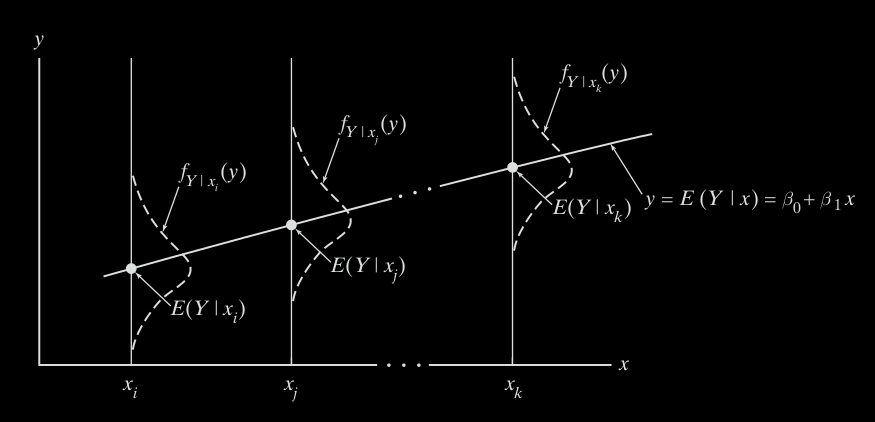
\includegraphics[align=c,height=1.22in]{Figure_11-3-2-neg.png}
\begin{minipage}{0.38\textwidth}
Drawing inferences on
	\begin{enumerate}
		\item the slope $\beta_1$\\[1em]
		\item the  intercept $\beta_0$ \\[1em]
		\item shape parameter $\sigma^2$ \\[1em]
		\item the regresion line itself
		\item[] $y = \E[Y|x]=\beta_0+\beta_1 x$\\[1em]
		\item the future observations\\[1em]
		\item testing two slopes.
	\end{enumerate}
\end{minipage}
\end{frame}
%-------------- end slide -------------------------------%}}}
%-------------- start slide -------------------------------%{{{ 10.59
\begin{frame}{1. Drawing inferences on $\beta_1$}
\begin{enumerate}
\item[Thm.]  $\displaystyle T_{n-2} = \frac{\hat\beta_1 - \beta_1}{S\bigg/\sqrt{\sum_{i=1}^n (x_i-\bar x)^2}}\sim $ Student t distribution with df $=n-2$.
\vfill
\item Hypothesis test $H_0:\beta_1=\beta_1'$ vs. ....\\[2em]
\item C.I. for $\beta_1$: \quad $\beta_{1e}\pm t_{\alpha/2,n-2} \frac{s}{\sqrt{\sum_{i=1}^n (x_i-\bar x)}}$
\end{enumerate}
\end{frame}
%-------------- end slide -------------------------------%}}}
%-------------- start slide -------------------------------%{{{ 10.60
\begin{frame}{2. Drawing inferences on $\beta_0$}
	\centering
	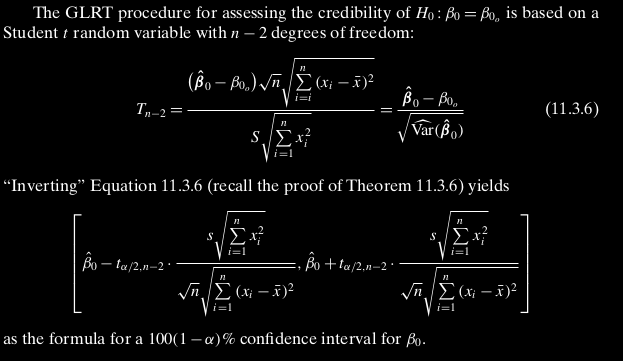
\includegraphics[scale=0.5]{Eq_11-3-6-neg.png}
\end{frame}
%-------------- end slide -------------------------------%}}}
%-------------- start slide -------------------------------%{{{ 10.61
\begin{frame}{3. Drawing inferences on $\sigma^2$}

	\centering
	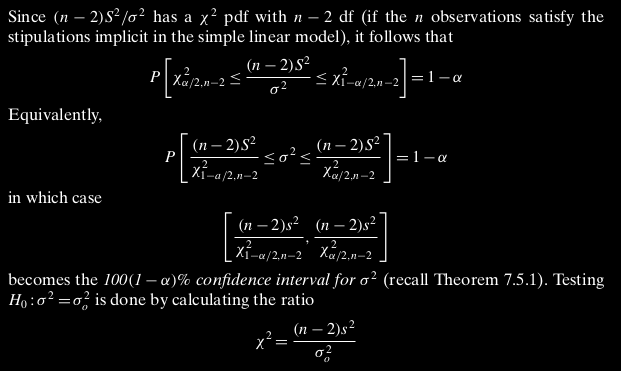
\includegraphics[scale=0.5]{Eq_11-3-6-2-neg.png}
	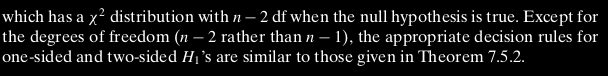
\includegraphics[scale=0.5]{Eq_11-3-6-3-neg.png}
\end{frame}
%-------------- end slide -------------------------------%}}}
%-------------- start slide -------------------------------%{{{ 10.62
\begin{frame}{4. Drawing inference on the regression line}

	\centering
	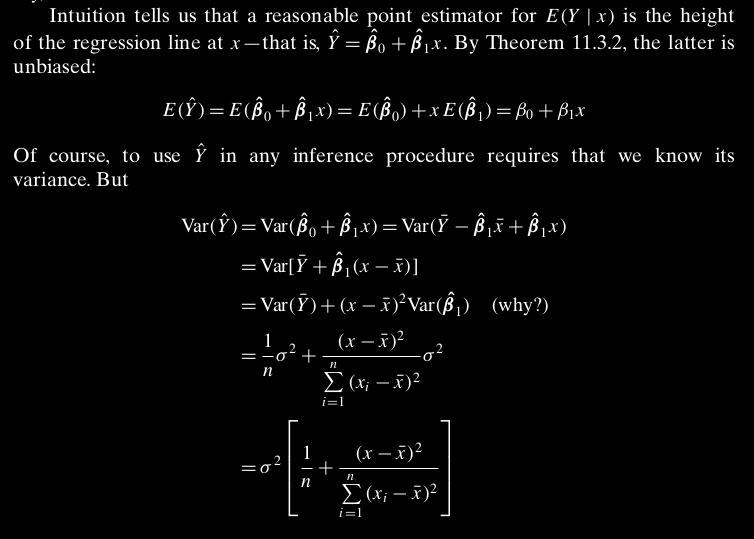
\includegraphics[scale=0.42]{Inference_EYX-1-neg.png}
\end{frame}
%-------------- end slide -------------------------------%}}}
%-------------- start slide -------------------------------%{{{ 10.63
\begin{frame}

	\centering
	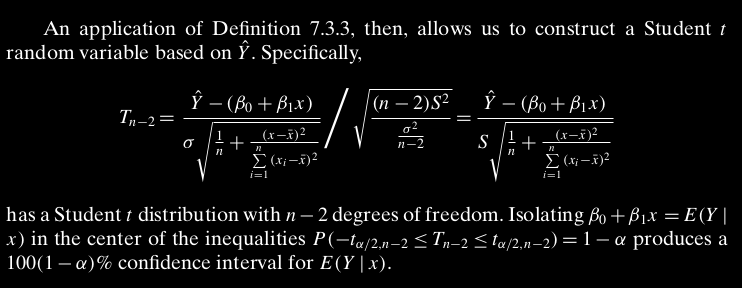
\includegraphics[scale=0.43]{Inference_EYX-2-neg.png}
\end{frame}
%-------------- end slide -------------------------------%}}}
%-------------- start slide -------------------------------%{{{ 10.64
\begin{frame}
	\centering
	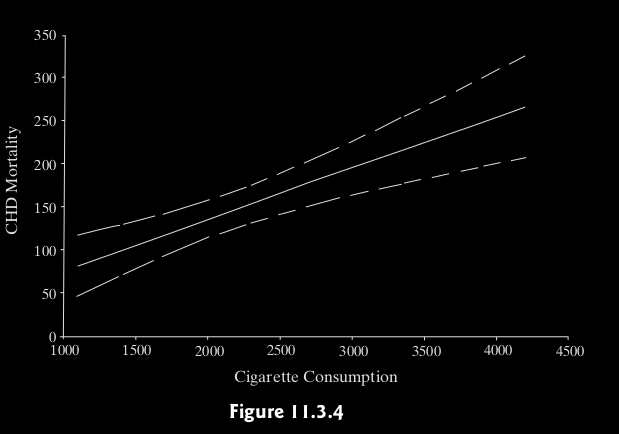
\includegraphics[scale=0.43]{Figure_11-3-4-neg.png}
\end{frame}
%-------------- end slide -------------------------------%}}}
%-------------- start slide -------------------------------%{{{ 10.65
\begin{frame}{5. Drawing inference on future observations}
\centering
	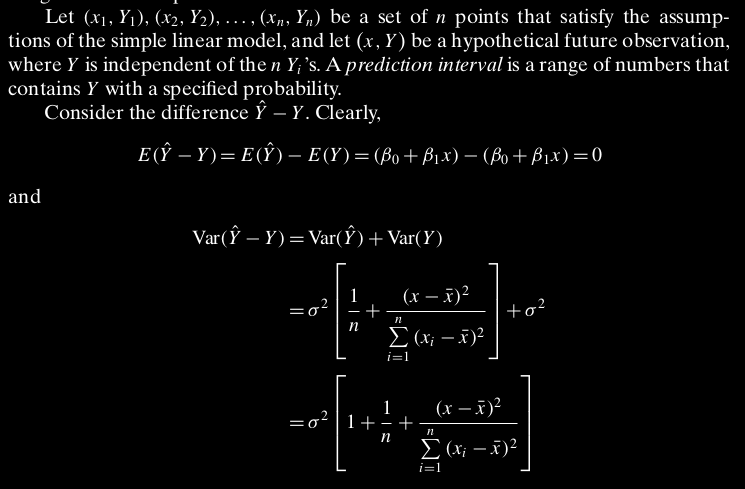
\includegraphics[scale=0.43]{Future_obs-1-neg.png}
\end{frame}
%-------------- end slide -------------------------------%}}}
%-------------- start slide -------------------------------%{{{ 10.66
\begin{frame}
\centering
	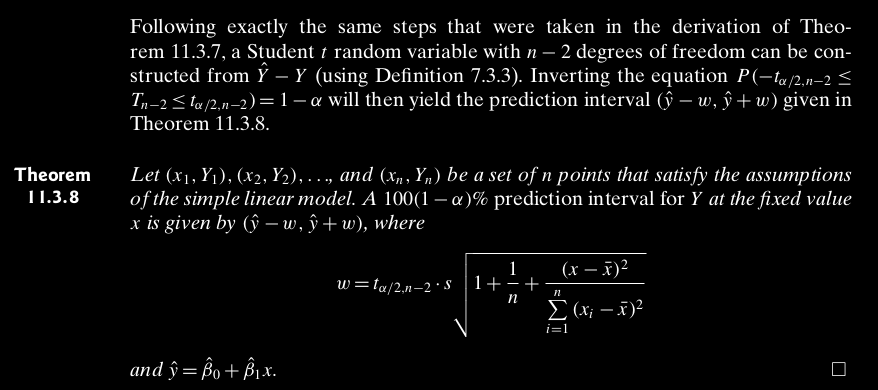
\includegraphics[scale=0.38]{Future_obs-2-neg.png}
\end{frame}
%-------------- end slide -------------------------------%}}}
%-------------- start slide -------------------------------%{{{ 10.67
\begin{frame}
\begin{enumerate}
\item[E.g. 1] Does smoking contribute to coronary heat disease?
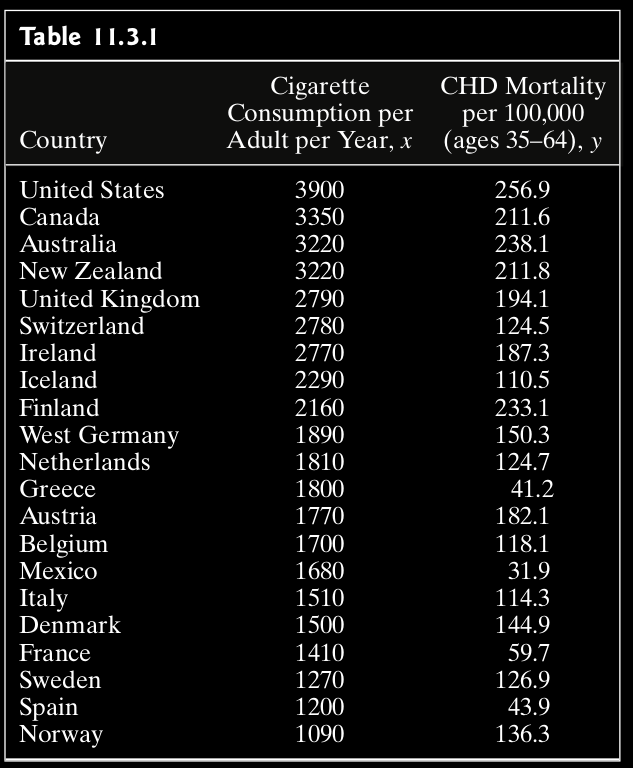
\includegraphics[scale=0.25]{Table_11-3-1-neg.png}
\item[]1) Test $H_0:\beta_1=0$ v.s. $H_1:\beta_1>0$ at $\alpha=0.05$.
\item[]2) Find C.I. for $\beta_1$ with the same $\alpha$.
\end{enumerate}
\end{frame}
%-------------- end slide -------------------------------%}}}
%-------------- start slide -------------------------------%{{{ 10.68
\begin{frame}[fragile]
	\begin{enumerate}
		\item[Sol.] \url{http://r-statistics.co/Linear-Regression.html}
			\vfill
		\item[1.] Let's first take of look of the data by scatter plot:
\begin{center}
\begin{minipage}{0.6\textwidth}
\begin{lstlisting}
scatter.smooth(x=x, y=y, main="Cigarette ~ Mortality")
\end{lstlisting}
\end{minipage}
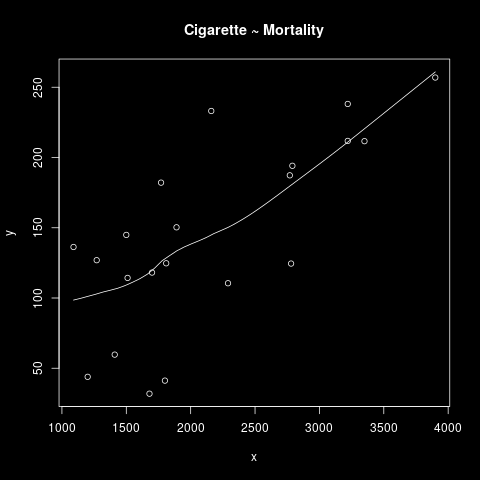
\includegraphics[scale=0.3]{Case_11-3-1-Scatter-neg.png}
\end{center}
\vfill
\item[] Suggests a linearly increasing relationship between $x$ and $y$.
	\end{enumerate}
\end{frame}
%-------------- end slide -------------------------------%}}}
%-------------- start slide -------------------------------%{{{ 10.69
\begin{frame}

	\begin{enumerate}
		\item[2.] Check outliers using boxplot.
			\vfill
			\begin{center}
				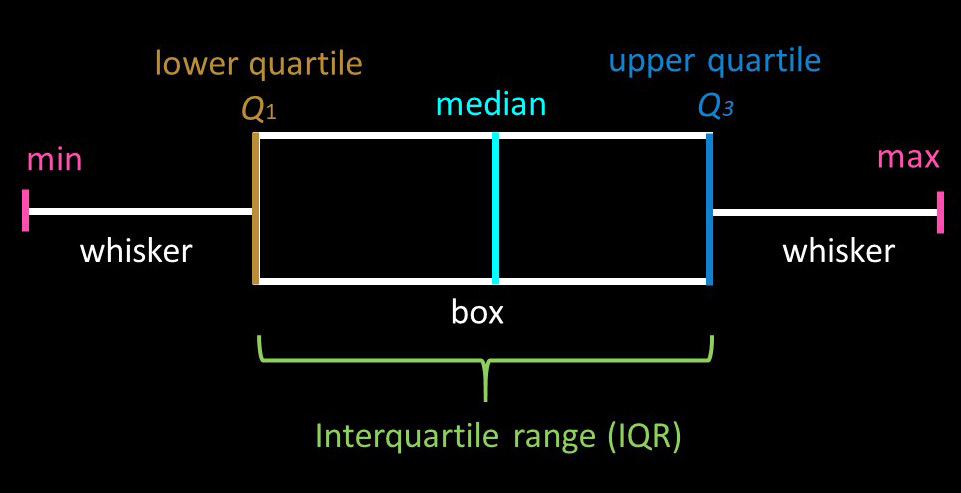
\includegraphics[scale=0.2]{boxplot-neg.jpg}
			\end{center}
			\vfill
		\item[] Any datapoint that lies outside the $r\times$IQR is considered an outlier.
			\\[1em]
			Generally, $r=1.5$.
			\end{enumerate}
	\end{frame} % }}}
%-------------- start slide -------------------------------%{{{ 10.70
\begin{frame}[fragile]


	\begin{center}
\begin{lstlisting}
r <- 1.5
par(mfrow=c(1, 2))  # divide graph area in 2 columns
boxplot(x, main="Cigarette", range=r, sub=paste("Outlier rows: ", boxplot.stats(x, coef=r)$out))  # box plot for 'Cigarette'
boxplot(y, main="Mortality", range=r, sub=paste("Outlier rows: ", boxplot.stats(y, coef=r)$out))  # box plot for 'Mortality'
\end{lstlisting}
\vfill
\begin{minipage}{0.45\textwidth}
\centering
$r=1.5$
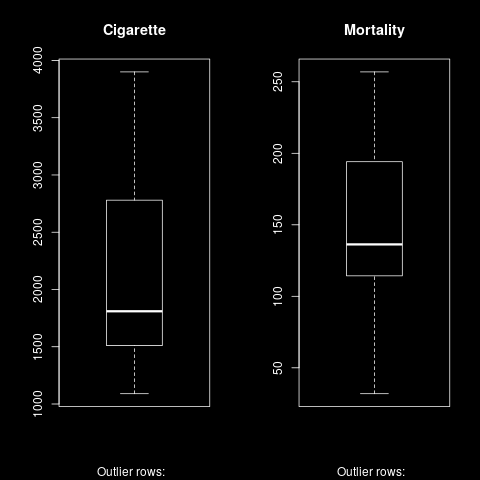
\includegraphics[scale=0.3]{Case_11-3-1-Outliers2-neg.png}
\end{minipage}
\hfill
\begin{minipage}{0.45\textwidth}
\centering
$r=1$
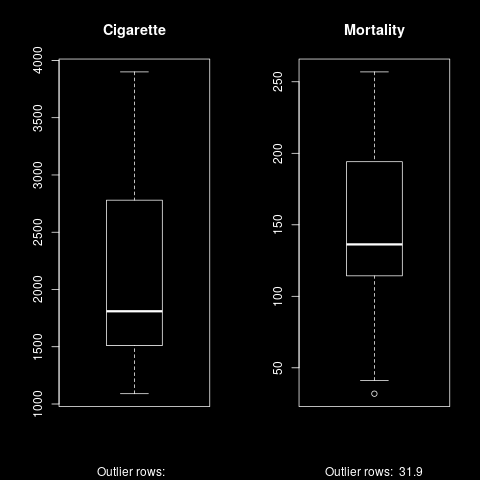
\includegraphics[scale=0.3]{Case_11-3-1-Outliers1-neg.png}
\end{minipage}
	\end{center}
\end{frame}
%-------------- end slide -------------------------------%}}}
%-------------- start slide -------------------------------%{{{ 10.71
\begin{frame}[fragile]
	\begin{enumerate}
		\item[3.] Compute kernel density estimates
\vfill
\begin{center}
	\begin{minipage}{0.95\textwidth}
\begin{lstlisting}
library(e1071)
plot(density(x), main="Density Plot: Cigarette", ylab="Frequency",
     sub=paste("Skewness:", round(e1071::skewness(x), 2)))  # density plot for 'Cigarette'
polygon(density(x), col="red")
plot(density(y), main="Density Plot: Mortality", ylab="Frequency",
     sub=paste("Skewness:", round(e1071::skewness(y), 2)))  # density plot for 'Mortality'
polygon(density(y), col="red")
\end{lstlisting}
\end{minipage}
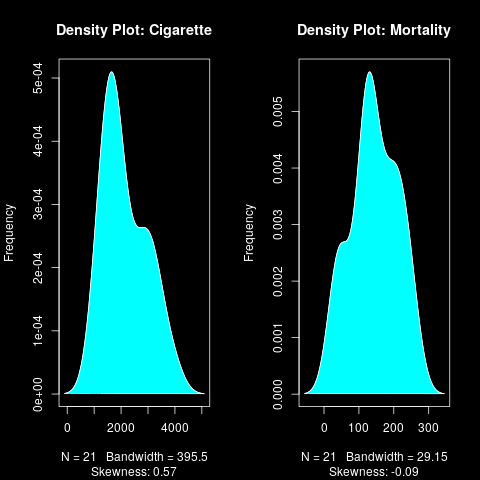
\includegraphics[scale=0.3]{Case_11-3-1-Density-neg.png}
\end{center}
	\end{enumerate}
\end{frame}
%-------------- end slide -------------------------------%}}}
%-------------- start slide -------------------------------%{{{ 10.72
\begin{frame}[fragile]

\begin{enumerate}
	\item[4.] Compute correlation coeficient. \\[2em]
	\item[]	Correlation is a statistical measure with values in $[-1,1]$ that suggests the level of linear dependence between two variables.\\[2em]
\item[] A value closer to 0 suggests a weak relationship between the variables. A low correlation $(-0.2, 0.2)$ probably suggests that much of variation of the response variable $Y$ is unexplained by the predictor $X$, in which case, we should probably look for better explanatory variables.
\vfill
\begin{center}
\begin{minipage}{0.3\textwidth}
\begin{lstlisting}
> cor(x,y)
[1] 0.7295154
\end{lstlisting}
\end{minipage}
\end{center}
\end{enumerate}
\end{frame}
%-------------- end slide -------------------------------%}}}
%-------------- start slide -------------------------------%{{{ 10.73
\begin{frame}[fragile]

	\begin{enumerate}
		\item[5.] Compute linear regression.
			\vfill
		\item[]
	\begin{minipage}{0.9\textwidth}
\begin{lstlisting}
> CigMort <- data.frame("Cigarette" = x, "Mortality" = y) # Build the data frame
> linearMod <- lm(Mortality ~ Cigarette, data=CigMort) # linear regression
> print(linearMod) # Print out the result

Call:
lm(formula = Mortality ~ Cigarette, data = CigMort)

Coefficients:
(Intercept)    Cigarette
    15.7711       0.0601
\end{lstlisting}
	\end{minipage}
	\vfill
\item[]
	\[
	y = 15.7711 + 0.0601 x
	\]
	\end{enumerate}
\end{frame}
%-------------- end slide -------------------------------%}}}
%-------------- start slide -------------------------------%{{{ 10.74
\begin{frame}[fragile]

	\begin{enumerate}
		\item[6.] Check statistical significance of the linear model
			\vfill
			\begin{center}
				\begin{minipage}{0.7\textwidth}
\begin{lstlisting}
> summary(linearMod)

Call:
lm(formula = Mortality ~ Cigarette, data = CigMort)

Residuals:
    Min      1Q  Median      3Q     Max
-84.835 -40.809   5.058  28.814  87.518

Coefficients:
            Estimate Std. Error t value Pr(>|t|)
(Intercept) 15.77115   29.57889   0.533 0.600085
Cigarette    0.06010    0.01293   4.649 0.000175 ***
---
Signif. codes:  0 "***" 0.001 "**" 0.01 "*" 0.05 "." 0.1 " " 1

Residual standard error: 46.71 on 19 degrees of freedom
Multiple R-squared:  0.5322,	Adjusted R-squared:  0.5076
F-statistic: 21.62 on 1 and 19 DF,  p-value: 0.0001749
\end{lstlisting}
				\end{minipage}
\end{center}
\vfill
\begin{enumerate}
\item By default, p-values are computed for $H_0: \beta_i=0$ vs. $H_1:\beta_i\ne 0$, $i=0,1$.
\item The more stars by the variable's p-Value, the more significant the variable.
\end{enumerate}
	\end{enumerate}
\end{frame}
%-------------- end slide -------------------------------%}}}
%-------------- start slide -------------------------------%{{{ 10.75
\begin{frame}[fragile]
	\vspace{2em}

	\begin{minipage}{0.45\textwidth}
	\begin{enumerate}
		\item[] Testing $H_0: \beta_1 = 0$ v.s. $H_1:\beta_1\ne 0$\\
		\item[] $t$-score is $4.4649$.
		\item[] $p$-value$=0.000175$
		\item[] Conclusion: reject at $\alpha=0.05$.
			\vspace{1em}
		\item[] $95\%$ C.I. for $\beta_1$:
	\end{enumerate}
	\end{minipage}
	\begin{minipage}{0.45\textwidth}
	\begin{enumerate}
		\item[] Testing $H_0: \beta_0 = 0$ v.s. $H_1:\beta_0\ne 0$\\
		\item[] $t$-score is $0.533$.
		\item[] $p$-value$=0.600$
		\item[] Conclusion: fail to reject at $\alpha=0.05$.
			\vspace{1em}
		\item[] $95\%$ C.I. for $\beta_0$:
	\end{enumerate}
	\end{minipage}
	\vfill
	\begin{center}
		\begin{minipage}{0.7\textwidth}
\begin{lstlisting}
> # 95% C.I. for slope parameter beta_1
> alpha <- 0.05
> for (i in c(1,0)) {
+   coef <- summary(linearMod)$coefficient
+   df <- linearMod$df.residual
+   lbd <- coef[i+1,1] - pt(1-alpha/2,df) * coef[i+1,2]
+   ubd <- coef[i+1,1] + pt(1-alpha/2,df) * coef[i+1,2]
+   print(paste("95% C.I. for the slope is beta_",i,
+               " is (", round(lbd,3), ",", round(ubd,3),")"))
+ }
[1] "95% C.I. for the slope is beta_ 1  is ( 0.049 , 0.071 )"
[1] "95% C.I. for the slope is beta_ 0  is ( -8.753 , 40.295 )"
\end{lstlisting}
		\end{minipage}
	\end{center}
\end{frame}
%-------------- end slide -------------------------------%}}}
%-------------- start slide -------------------------------%{{{ 10.76
\begin{frame}[fragile]

	\begin{enumerate}
		\item[7.] Compute R-Squared and the adjusted R-Squared.
			\vfill
		\item[]
			\[
				R^2 = 1-\frac{SSE}{SST} \quad \text{and}\quad
				R^2_{adj} = 1-\frac{MSE}{MST}
		\]
		\vfill
		\item[]
			\begin{center}
				\begin{minipage}{0.7\textwidth}
\begin{lstlisting}
> names(summary(linearMod))
 [1] "call"          "terms"         "residuals"     "coefficients"
 [5] "aliased"       "sigma"         "df"            "r.squared"
 [9] "adj.r.squared" "fstatistic"    "cov.unscaled"
> summary(linearMod)$r.squared
[1] 0.5321927
> summary(linearMod)$adj.r.squared
[1] 0.5075712
\end{lstlisting}
				\end{minipage}
			\end{center}
			\vfill
		\item[] The large $r^2$ or $r^2_{adj}$ the better, the more powerful or expressive is the L.M.
\end{enumerate}
\end{frame}
%-------------- end slide -------------------------------%}}}
%-------------- start slide -------------------------------%{{{ 10.77
\begin{frame}[fragile]

	\begin{enumerate}
		\item[8.] Residue standard error and $F$-statistic
			\vfill
		\item[]
			\[
				\text{Residue standard error} = \sqrt{MSE} = \sqrt{\frac{SSE}{n-q}}
			\]
\vfill
		\item[]
			\[
				F = \frac{MSR}{MSE} = \frac{SSR/(q-1)}{SSE/(n-q)}\sim \text{F-distribution $(df_1 = q-1, df_2 = n-q)$ }
			\]
\vfill
\item[]
	\begin{center}
		\begin{minipage}{0.7\textwidth}
\begin{lstlisting}
> names(summary(linearMod))
 [1] "call"          "terms"         "residuals"     "coefficients"
 [5] "aliased"       "sigma"         "df"            "r.squared"
 [9] "adj.r.squared" "fstatistic"    "cov.unscaled"
> summary(linearMod)$sigma
[1] 46.70826
> summary(linearMod)$fstatistic
   value    numdf    dendf
21.61501  1.00000 19.00000
> f <- summary(linearMod)$fstatistic
> pf(f[1], f[2], f[3], lower=FALSE)
       value
0.0001748805
\end{lstlisting}
		\end{minipage}
	\end{center}
	\end{enumerate}
\end{frame}
%-------------- end slide -------------------------------%}}}
%-------------- start slide -------------------------------%{{{ 10.78
\begin{frame}[fragile]

	\begin{enumerate}
		\item[9.] Model selection:\\[2em]
		\item[]
			\begin{minipage}{0.45\textwidth}
\centering
 Akaike's information criterion \\
  --- AIC (Akaike, 1974)
		\[
			AIC = -2 \ln(\widehat{L}) +2 q
		\]
			\end{minipage}
			\begin{minipage}{0.45\textwidth}
Bayesian information criterion\\
--- BIC (Schwarz, 1978)
			\[
				BIC = -2 \ln(\widehat{L}) + q \ln(n)
			\]
			\end{minipage}
			\vfill
		\item[] $\widehat{L}$: the maximum of likelihood.
		\item[] $q$: the number of parameters in the model.
		\item[] $n$: the sample size.
			\vfill
		\item[]
			\begin{center}
				\begin{minipage}{0.3\textwidth}
\begin{lstlisting}
> AIC(linearMod)
[1] 224.9383
> BIC(linearMod)
[1] 228.0719
\end{lstlisting}
				\end{minipage}
				\vfill
		The lower the better!
			\end{center}
	\end{enumerate}
\end{frame}
%-------------- end slide -------------------------------%}}}
%-------------- start slide -------------------------------%{{{ 10.79
\begin{frame}

	\begin{enumerate}
		\item[10.] Does L.M. fit our model?
			\vfill
			\renewcommand{\arraystretch}{1.6}
			\begin{center}
				\begin{tabular}{ccc}
\hline
Statistic & criterion & our case\\
\hline
$R^2$ & Higher the better (>0.7) & $0.53$\\
$R^2_{adj}$ & Higher the better & $0.51$ \\
AIC & Lower the better & $225$\\
BIC & Lower the better & $228$\\
$\vdots$ & $\vdots$ & $\vdots$\\
\hline
				\end{tabular}
			\end{center}
	\end{enumerate}
\end{frame}
%-------------- end slide -------------------------------%}}}
%-------------- start slide -------------------------------%{{{ 10.80
\begin{frame}[fragile]

	\begin{enumerate}
		\item[11.] Drawing inference on $\E(Y|x)$\\[1em]
		\item[] Find $95\%$ C.I. for $Y$ at $x=4200$.
			\vfill
		\item[]
			\begin{center}
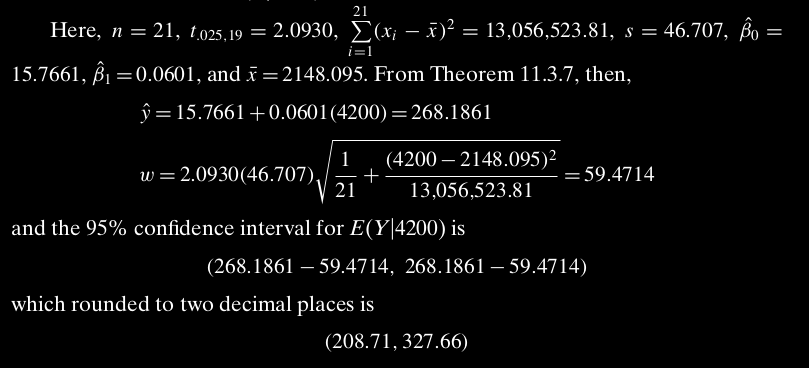
\includegraphics[scale=0.35]{Example_11-3-2-neg.png}
			\end{center}
	\end{enumerate}
\end{frame}
%-------------- end slide -------------------------------%}}}
%-------------- start slide -------------------------------%{{{ 10.81
\begin{frame}[fragile]
\begin{center}
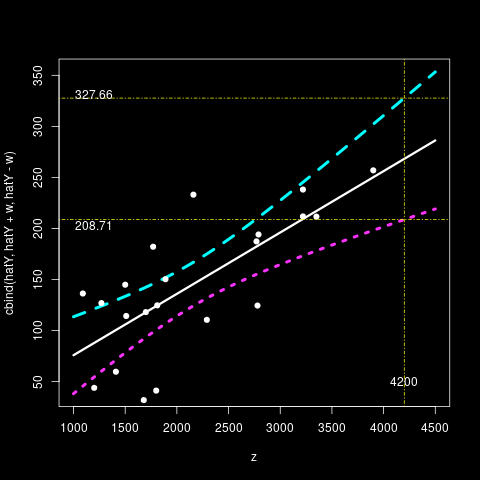
\includegraphics[scale=0.5]{EYX-neg.png}
\end{center}
\end{frame}
%-------------- end slide -------------------------------%}}}
%-------------- start slide -------------------------------%{{{ 10.82
\begin{frame}[fragile]
	\begin{center}
	\begin{minipage}{0.8\textwidth}
\begin{lstlisting}
s <- summary(linearMod)$sigma
beta <- linearMod$coefficients
z <- seq(1000,4500,1)
hatY <- beta[1]+beta[2]*z
w <- qt(0.975,19) * s * sqrt(1/21+(z-mean(x))^2/(sum((x-mean(x))^2)))
matplot(z,cbind(hatY,hatY+w,hatY-w),type = c("l","l","l"),lwd=c(3,4,4))
points(x, y, pch = 19)
abline(v=4200,col = "blue", lty = 4)
abline(h=208.71,col = "blue", lty = 4)
abline(h=327.66,col = "blue", lty = 4)
text(4200,50,4200)
text(1200,203,208.71)
text(1200,331,327.66)
\end{lstlisting}
\end{minipage}
	\end{center}
\end{frame}
%-------------- end slide -------------------------------%}}}
%-------------- start slide -------------------------------%{{{ 10.83
\begin{frame}[fragile]

	\begin{enumerate}
		\item[12.] Drawing inference on future observations.\\[1em]
		\item[] Find $95\%$ prediction interval for $Y$ at $x=4200$.
			\vfill
		\item[]
\begin{center}
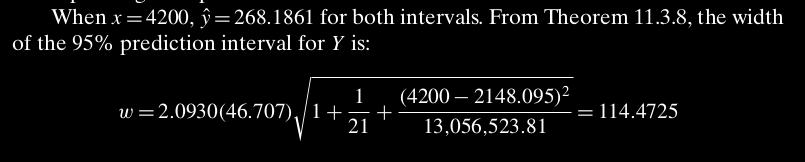
\includegraphics[scale=0.35]{Example_11-3-2-1-neg.png}
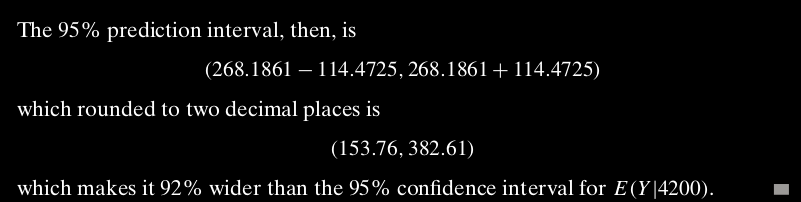
\includegraphics[scale=0.35]{Example_11-3-2-2-neg.png}
\end{center}
	\end{enumerate}
\end{frame}
%-------------- end slide -------------------------------%}}}
%-------------- start slide -------------------------------%{{{ 10.84
\begin{frame}[fragile]
\begin{center}
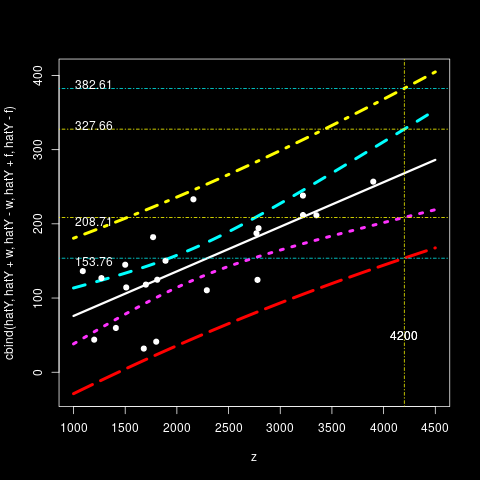
\includegraphics[scale=0.5]{EYX_Pred-neg.png}
\end{center}
\end{frame}
%-------------- end slide -------------------------------%}}}
%-------------- start slide -------------------------------%{{{ 10.85
\begin{frame}[fragile]
\begin{center}
\begin{minipage}{0.8\textwidth}
\begin{lstlisting}
s <- summary(linearMod)$sigma
beta <- linearMod$coefficients
z <- seq(1000,4500,1)
hatY <- beta[1]+beta[2]*z
w <- qt(0.975,19) * s * sqrt(1/21+(z-mean(x))^2/(sum((x-mean(x))^2)))
f <- qt(0.975,19) * s * sqrt(1+1/21+(z-mean(x))^2/(sum((x-mean(x))^2)))
matplot(z,cbind(hatY,hatY+w,hatY-w,hatY+f,hatY-f),
        type = c("l","l","l","l","l"),lwd=c(3,4,4,4,4))
points(x, y, pch = 19)
abline(v=4200,col = "blue", lty = 4)
abline(h=208.71,col = "blue", lty = 4)
abline(h=327.66,col = "blue", lty = 4)
text(4200,50,4200)
text(1200,208.71-5,208.71)
text(1200,327.66+5,327.66)
abline(h=153.76,col = "red", lty = 4)
abline(h=382.61,col = "red", lty = 4)
text(4200,50,4200)
text(1200,153.76-5,153.76)
text(1200,382.61+5,382.61)
\end{lstlisting}
		\end{minipage}
	\end{center}
\end{frame}
%-------------- end slide -------------------------------%}}}
%-------------- start slide -------------------------------%{{{ 10.86
\begin{frame}[fragile]

	\begin{enumerate}
		\item[13.] More about diagnozing the linear model:
			\vfill
		\item[]
			\begin{center}
				\begin{minipage}{0.7\textwidth}
\begin{lstlisting}
# diagnostic plots
layout(matrix(c(1,2,3,4),2,2)) # optional 4 graphs/page
plot(linearMod)
\end{lstlisting}
\end{minipage}
\end{center}
	\end{enumerate}
\end{frame}
%-------------- end slide -------------------------------%}}}
%-------------- start slide -------------------------------%{{{ 10.87
\begin{frame}[fragile]
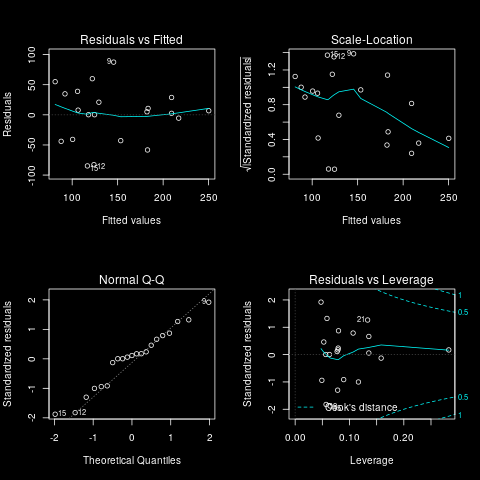
\includegraphics[scale=0.6]{diagnostic_plots-neg.png}
\end{frame}
%-------------- end slide -------------------------------%}}}
%-------------- start slide -------------------------------%{{{ 10.88
\begin{frame}
	\begin{enumerate}
		\item[E.g. 2] Find 95\% C.I. for the amount of increas year-by-year in the cost of Toyota Camry sedan. \\[2em]
			\begin{center}
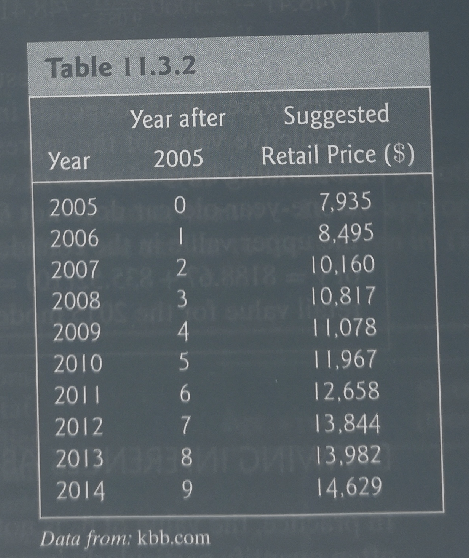
\includegraphics[scale=0.25]{Table_11-3-2-neg.png}
			\end{center}
	\end{enumerate}
\end{frame}
%-------------- end slide -------------------------------%}}}
%-------------- start slide -------------------------------%{{{ 10.89
\begin{frame}

	\begin{enumerate}
		\item[Sol.] We first find the regression:
			\vfill
			\begin{center}
				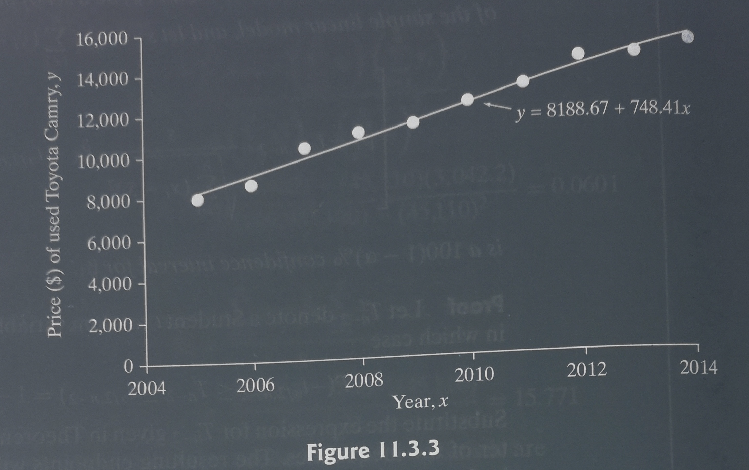
\includegraphics[scale=0.25]{Figure_11-3-3-neg.png}
			\end{center}
	\end{enumerate}
\end{frame}
%-------------- end slide -------------------------------%}}}
%-------------- start slide -------------------------------%{{{ 10.90
\begin{frame}
\centering
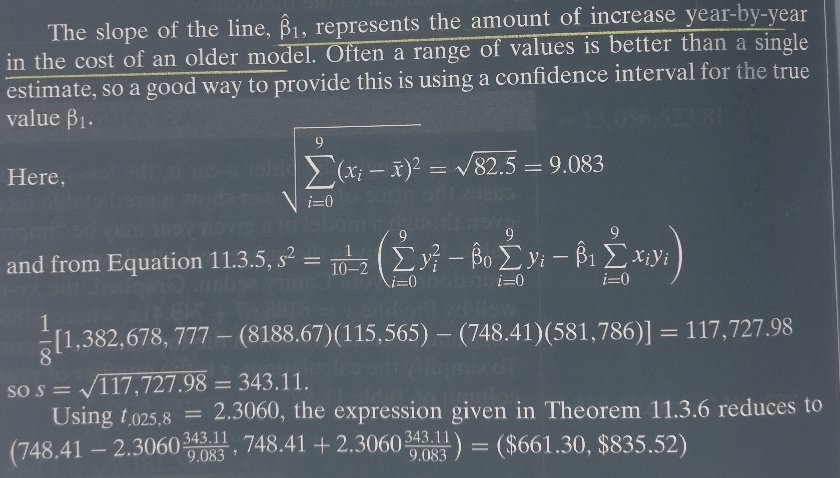
\includegraphics[scale=.35]{Case_11-3-2-Sol-neg.png}
\end{frame}
%-------------- end slide -------------------------------%}}}
%-------------- start slide -------------------------------%{{{ 10.91
\begin{frame}
	{7. Testing the equality of two slopes}
\centering
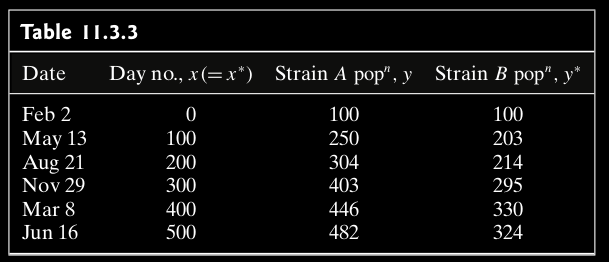
\includegraphics[scale=0.2,align=c,height=0.5in]{Table_11-3-3-neg.png}
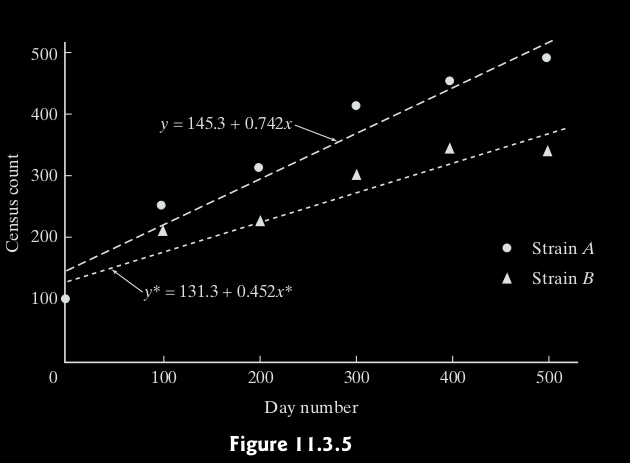
\includegraphics[scale=0.2,align=c,height=0.7in]{Figure_11-3-5-neg.png}\\
\vfill
Do you believe that $\beta_1 = \beta_1^*$?\\[2em]
Or is $\beta_1>\beta_1^*$ statisically significantly?
\end{frame}
%-------------- end slide -------------------------------%}}}
%-------------- start slide -------------------------------%{{{ 10.92
\begin{frame}
	\centering
	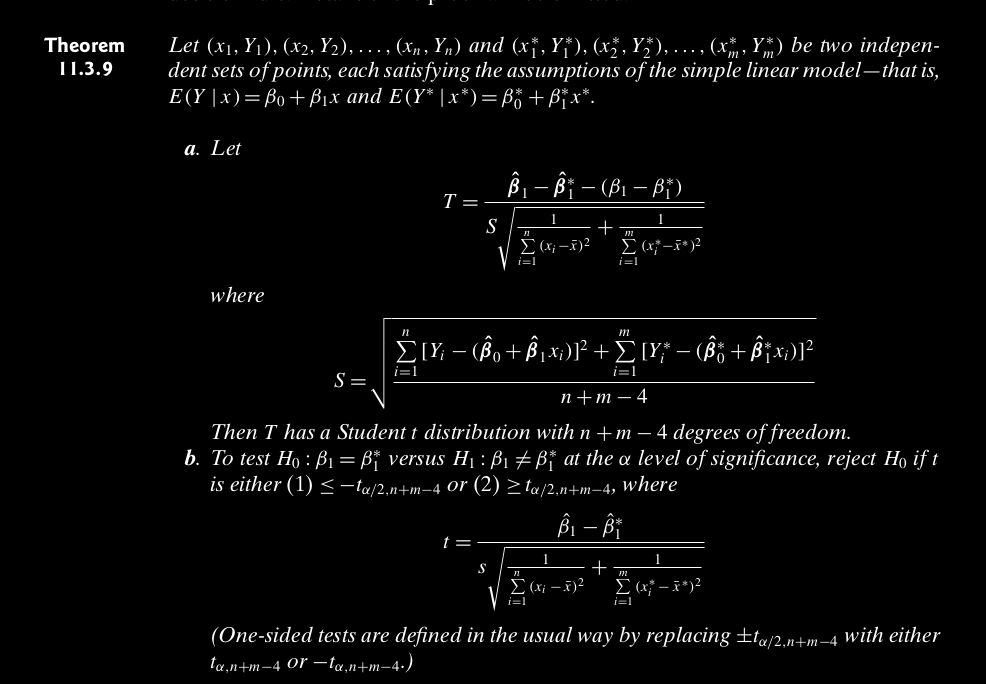
\includegraphics[scale=0.32]{Theorem_11-3-9-neg.png}
\vfill \pause
$S^2 = SSE$ and $q = 4$.
\end{frame}
%-------------- end slide -------------------------------%}}}
%-------------- start slide -------------------------------%{{{ 10.93
\begin{frame}

	\begin{enumerate}
		\item[Sol.] Test
			\[
				H_0: \beta_1 = \beta_1^* \quad\text{v.s.}\quad
				H_1: \beta_1 > \beta_1^*.
			\]
			\vfill
		\item[] Long computations  ... $t = 2.50$.
			\begin{center}
				\url{http://math.emory.edu/~lchen41/teaching/2020_Spring/Ex_11-3-4.R}
			\end{center}
			\vfill
		\item[] Critical region: $t>t_{0.05,8} = 1.8595$.
			\vfill
		\item[] Reject. \myEnd
	\end{enumerate}
\end{frame}
%-------------- end slide -------------------------------%}}}
%-------------- start slide -------------------------------%{{{ 10.94
\begin{frame}[fragile]
	\begin{center}
\begin{lstlisting}
> # Example 11.3.4
> # Read data first
> Input <- ("
+ x     yA    yB
+ 0     100   100
+ 100   250   203
+ 200   304   214
+ 300   403   295
+ 400   446   330
+ 500   482   324
+ ")
> Data = read.table(textConnection(Input),
+                   header=TRUE)
> Data
    x  yA  yB
1   0 100 100
2 100 250 203
3 200 304 214
4 300 403 295
5 400 446 330
6 500 482 324
\end{lstlisting}
	\end{center}
\end{frame}
%-------------- end slide -------------------------------%}}}
%-------------- start slide -------------------------------%{{{ 10.95
\begin{frame}[fragile]
\begin{lstlisting}
> #fit the first model ...
> DataA <- data.frame(x = Data$x,yA = Data$yA)
> fitA <- lm(yA~x, DataA)
> summary(fitA)

Call:
lm(formula = yA ~ x, data = DataA)

Residuals:
      1       2       3       4       5       6
-45.333  30.467  10.267  35.067   3.867 -34.333

Coefficients:
             Estimate Std. Error t value Pr(>|t|)
(Intercept) 145.33333   26.86684   5.409  0.00566 **
x             0.74200    0.08874   8.362  0.00112 **
---
Signif. codes:  0 '***' 0.001 '**' 0.01 '*' 0.05 '.' 0.1 ' ' 1

Residual standard error: 37.12 on 4 degrees of freedom
Multiple R-squared:  0.9459,	Adjusted R-squared:  0.9324
F-statistic: 69.92 on 1 and 4 DF,  p-value: 0.001119
\end{lstlisting}
\end{frame}
%-------------- end slide -------------------------------%}}}
%-------------- start slide -------------------------------%{{{ 10.96
\begin{frame}[fragile]
\begin{lstlisting}
> #fit the second model ...
> DataB <- data.frame(x = Data$x,yB = Data$yB)
> fitB <- lm(yB~x, DataB)
> summary(fitB)

Call:
lm(formula = yB ~ x, data = DataB)

Residuals:
      1       2       3       4       5       6
-31.333  26.467  -7.733  28.067  17.867 -33.333

Coefficients:
             Estimate Std. Error t value Pr(>|t|)
(Intercept) 131.33333   22.77255   5.767  0.00449 **
x             0.45200    0.07522   6.009  0.00386 **
---
Signif. codes:  0 '***' 0.001 '**' 0.01 '*' 0.05 '.' 0.1 ' ' 1

Residual standard error: 31.46 on 4 degrees of freedom
Multiple R-squared:  0.9003,	Adjusted R-squared:  0.8754
F-statistic: 36.11 on 1 and 4 DF,  p-value: 0.00386
\end{lstlisting}
\end{frame}
%-------------- end slide -------------------------------%}}}
%-------------- start slide -------------------------------%{{{ 10.97
\begin{frame}[fragile]
\begin{lstlisting}
> # Now compute t-score and p-value
> sA <- summary(fitA)$coefficients
> sA
            Estimate  Std. Error  t value    Pr(>|t|)
(Intercept) 145.3333 26.86683800 5.409395 0.005656733
x             0.7420  0.08873825 8.361671 0.001118570
> sB <- summary(fitB)$coefficients
> sB
            Estimate  Std. Error  t value    Pr(>|t|)
(Intercept) 131.3333 22.77254682 5.767178 0.004486443
x             0.4520  0.07521525 6.009420 0.003860274
> db <- (sA[2,1]-sB[2,1]) # difference of beta_1's
> db
[1] 0.29
> sd <- sqrt(sB[2,2]^2+sA[2,2]^2) # standard deviation
> sd
[1] 0.1163263
> df <- (fitA$df.residual+fitB$df.residual) # degrees of freedom
> df
[1] 8
> td <- db/sd # t-score
> pv <- 2*pt(-abs(td), df) # two-sided p-value
> print(paste("t-score is ", round(td,3),
+             "and p-value is", round(pv,3)))
[1] "t-score is  2.493 and p-value is 0.037"
\end{lstlisting}
\end{frame}
%-------------- end slide -------------------------------%}}}
%-------------- start slide -------------------------------%{{{ 10.98
\begin{frame}[fragile]{
	\dangersign[5ex]\\
You should always visualize your data \\
before any analysis}
	\begin{center}
		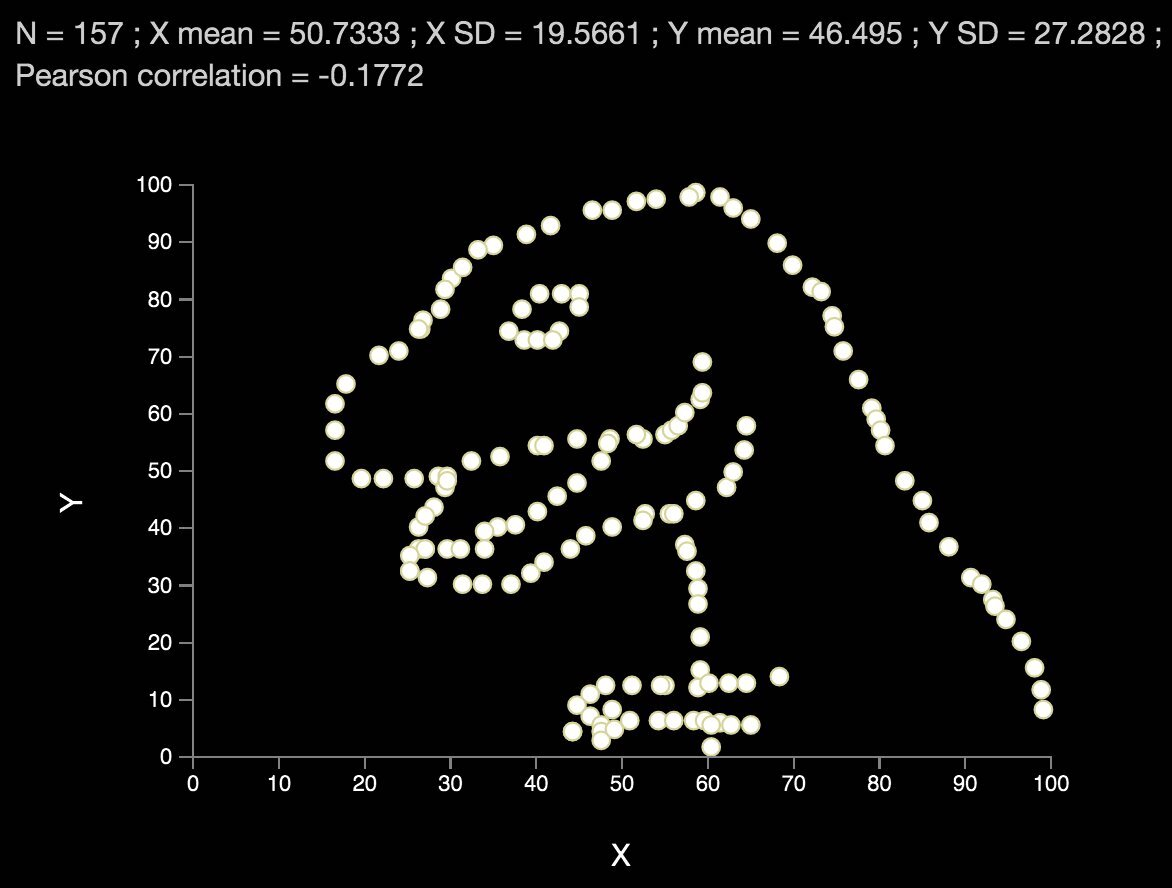
\includegraphics[scale=0.2]{Datasarous-neg.jpg}
	\end{center}
\end{frame}
%-------------- end slide -------------------------------%}}}

\mySection{11.4 Covariance and Correlation}
%-------------- start slide -------------------------------%{{{ 11.9
\begin{frame}
	% {\S\: 11.4  Covariance and Correlation}
	\centering
	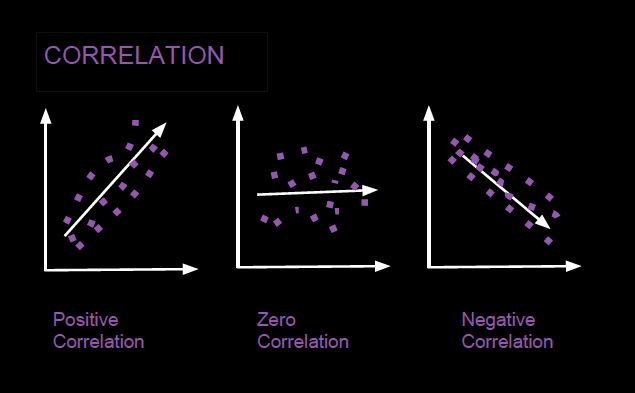
\includegraphics[scale=0.5]{Correlation_coefficent-neg.png}
\end{frame}
%-------------- end slide -------------------------------%}}}
%-------------- start slide -------------------------------%{{{ 11.10
\begin{frame}
	\centering
	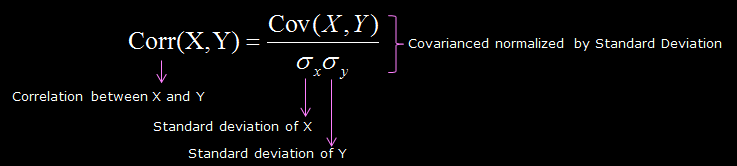
\includegraphics[scale=0.4]{Correlation_coefficent_Formula-neg.png}
\vfill

\begin{enumerate}
	\item[] Notation: $Corr(X,Y) = \rho(X,Y) = \rho_{XY}$\\[3em]
	\item[] Computing:  $\Var(X) = \sigma_X^2$, $\Var(Y)=\sigma_Y^2$, $\Cov(X,Y)=\sigma_{XY}$
	\item[]
		\[
			\Downarrow
		\]
		\[
			\rho_{XY} = \frac{\sigma_{XY}}{\sigma_X\sigma_Y}
		\]
\end{enumerate}
\end{frame}
%-------------- end slide -------------------------------%}}}
%-------------- start slide -------------------------------%{{{ 11.11
\begin{frame}

	\begin{enumerate}
		\item[Thm.] For any two random variables $X$ and $Y$,
		\item[a.] $|\rho(X,Y)| \le 1$
		\item[b.] $\rho(X,Y) = 1$ if and only if $Y=aX+b$ for some $a>0$ and $b\in\R$;
		\item[] $\rho(X,Y) = -1$ if and only if $Y=aX+b$ for some $a<0$ and $b\in\R$.
			\vfill
		\item[Proof.] (a)
			\begin{gather*}
				| \rho(X,Y) | \le 1 \\[1em]
				\Updownarrow
			\end{gather*}
			\begin{align*}
				\left| \E\left((X-\E(X))(Y-\E(Y))\right) \right| &\le \sqrt{\Var(X)\Var(Y)}\\
																												 &= \sqrt{\E\left((X-\E(X))^2\right)} \sqrt{\E\left((Y-\E(Y))^2\right)}
			\end{align*}
			which is nothing but the Cauchy-Schwartz inequality.
	\end{enumerate}
\end{frame}
%-------------- end slide -------------------------------%}}}
%-------------- start slide -------------------------------%{{{ 1
\begin{frame}[fragile]
\begin{itemize}
	\item[] (b) In the Cauchy-Schwartz inequality, the equality holds if and only if for some $a\ne 0$,
		\begin{align*}
			X-\E(X) = a [Y - E(Y)]
		\end{align*}
		namely,
		\begin{align*}
			X = a Y + b,\qquad \text{with}\quad b= \E(X) -a \E(Y).
		\end{align*}
	\item[] In particular, $a>0$ corresponds to the case $\rho(X,Y)=1$ and $a<0$ to $\rho(X,Y)=-1$.
		\myEnd
\end{itemize}
\end{frame}
%-------------- end slide -------------------------------%}}}l
%-------------- start slide -------------------------------%{{{ 11.12
\begin{frame}{Estimating $\rho(X,Y)$\\
	-- Sample correlation coefficient}

	\begin{enumerate}
		\item[]
	\begin{align*}
		\rho(X,Y) &=  \frac{\Cov(X,Y)}{\sqrt{\Var(X)}\sqrt{\Var(Y)}}\\[2em]
& =  \frac{\E[X Y] -\E[X]\E[Y]}{\sqrt{\E[X^2]-\E[X]^2}\sqrt{\E[Y^2]-\E[Y]^2}}
	\end{align*}
	\vfill
\item[] \[\Downarrow\]
	\vfill
\item[]
	\[
		R =  \frac{n\sum_{i=1}^n X_iY_i -\left(\sum_{i=1}^n X_i \right )\left(\sum_{i=1}^n Y_i \right ) }{\sqrt{n\sum_{i=1}^n X_i^2- \left(\sum_{i=1}^n X_i \right )^2}\sqrt{n\sum_{i=1}^n Y_i^2- \left(\sum_{i=1}^n Y_i \right )^2}}
	\]
	\vfill
\item[]
	\begin{center}
		{\it \textcolor{yellow}{Pearson product-moment correlation coefficient}}\\[1em]
	or \\[1em]
	{\it \textcolor{yellow}{Sample correlation coefficient}}
	\end{center}
	\end{enumerate}
\end{frame}
%-------------- end slide -------------------------------%}}}
%-------------- start slide -------------------------------%{{{ 11.13
\begin{frame}

	\begin{enumerate}
		\item[Thm.] $$R^2 = 1 - \frac{SSE}{SST} = \frac{SST-SSE}{SST} = \frac{SSTR}{SST} $$ where
			\[
				SSE = \sum_{i=1}^n \left(Y_i - \widehat{Y}_i \right)^2, \quad \widehat{Y_i} = \hat{\beta}_0+\hat{\beta}_1 X_i
			\]
			\[
				SST =  \sum_{i=1}^n \left(Y_i - \overline{Y}_i \right)^2, \quad\text{and}\quad
				SSTR = SST-SSE.
			\]
			\vfill
		\item[Remark] SSE: sum of square errors $\sim$ the variation in $y_i$'s not explained by L.M.\\[1em]
		\item[] SST: Total sum of squares $\sim$ total variability. \\[1em]
		\item[] SSTR: Treatment sum of sqrs. $\sim$ the variation in $y_i$'s explained by L.M. \\[1em]
		\item[] $R^2$ (or $r^2$ when $X_i$ and $Y_i$ are replaced by $x_i$ and $y_i$) $\sim$ proportion of total variation in the $y_i$'s that can be attributed to L.M.  \\
		\item[]
			\begin{center}
			{\it Coefficient of determination} or simply {\it R squared}
			\end{center}
	\end{enumerate}
\end{frame}
%-------------- end slide -------------------------------%}}}
%-------------- start slide -------------------------------%{{{ 11.14
\begin{frame}
	\OneFrame{Proof}
\end{frame}
%-------------- end slide -------------------------------%}}}
%-------------- start slide -------------------------------%{{{ 11.15
\begin{frame}{Adjusted R-squared}

	\begin{enumerate}
		\item[Def.] The adjusted R-squareed:
	\[
		R^2_{adj} := 1-\frac{MSE}{MST}
	\]
where
\[
	MSE = \frac{SSE}{n-q} \qquad\text{and}\qquad MST = \frac{SST}{n-1}
\]
and $q$ is number of parameters in the model.
\vfill
\item[Relation:]
	\[
		R^2_{adj} = 1- \left(1-R^2\right) \frac{n-1}{n-q}
	\]
	\vfill
\item[] MSE: Mean squared error.
\item[] MST: Mean squared total.
\item[] MSR = MSTR: Mean square for treatment (or regresssion).
	\[
		MSR = MSTR = \frac{SSTR}{q-1}
	\]
	\end{enumerate}
\end{frame}
%-------------- end slide -------------------------------%}}}

\mySection{11.5 The Bivariate Normal Distribution}
%-------------- start slide -------------------------------%{{{
\begin{frame}{\S\: 11.5 The Bivariate Normal Distribution}
\end{frame}
%-------------- end slide -------------------------------%}}}


\end{document}

